\documentclass[fontsize = 12pt, paper = a4]{scrreprt} 

\setlength{\parindent}{0pt}
\usepackage[english,ngerman]{babel}
\usepackage[utf8]{inputenc} 
\usepackage{enumerate}
\usepackage{amssymb,amsmath}

%------------ Überschriften verkleinern und hochsetzen ----------%

%\makeatlettern
%\renewcommand*\@makechapterhead[1]{%
%{\parindent \z@ \raggedright \normalfont
%\LARGE\bfseries
%\ifnum \c@secnumdepth >\m@ne
%\thechapter\space
%\fi
%#1\par\nobreak
%\vskip 20\p@
%}} 

% ------------------------ Blattlayout- -------------------------%

\usepackage {geometry}   
\geometry   {left     = 2.5cm,
             right    = 2.5cm, 
             top      = 1.5cm,
             bottom   = 1.5cm,
             includehead, includefoot}
             
% ------------------------ Seitenstil ---------------------------%           

% Umdefinieren von Befehlen zur Vermeidung von Bugs:

\renewcommand*{\chapterpagestyle}{scrheadings} 
\renewcommand*{\chapterheadstartvskip}{\vspace*{-\topskip}}

% Gestaltung der Kopf- und Fußzeile:

\pagenumbering{arabic}
            
\usepackage[automark]{scrpage2}
\automark[chapter]{section}
\pagestyle{scrheadings} 
\ohead[\pagemark]{\pagemark}
\setlength{\footskip}{5mm} 

\clearscrheadfoot
\lohead{Entwurfsdokument}
\rohead{\headmark}
\lofoot{Softwareprojekt TU Ilmenau SS 2013}
\rofoot{\pagemark}

% Kopf- und Fußzeilenlinie:

\setheadsepline{.6pt} % Linie für Kopfzeile
\setfootsepline{.6pt} % Linie für Fußzeile 

% Für Unterstreichungen:

\usepackage[normalem]{ulem}

% Buchstabenglättung am Rand:
  
\usepackage {microtype} 

% Bildunterschriften zentrieren:

%\usepackage{caption}
%\captionsetup{margin=10pt,font=small,labelfont=bf, justification = centering}

%-------------------------------------------------------------------%

% Für die Einbindung von Bildern:

\usepackage[pdftex]{graphicx} % .pdf, .png oder .jpg möglich!
\usepackage{rotating}         % Grafiken rotieren

% Nutzung in drei Umgebungen möglich:

% (1) \begin{turn}{Winkel} ...  \end{turn}
% (2) \begin{sideways} ... \end{sideways} 90° im math. pos. Sinn
% (3) \begin{rotate}{Winkel} ... \end{rotate} 
%     ---> 90° im math. pos. Sinn, allerdings keine Platzreservierung 

\usepackage{wrapfig}
%\usepackage{picins}   % Textumflossene Grafiken
\usepackage{subfigure}
\usepackage{floatflt}
\usepackage[justification=centering]{caption}

%-------------------------------------------------------------------%
 
% Packete für Tabellen:

\usepackage{booktabs}
\usepackage{array}    % optional
\usepackage{tabularx} % optional

\usepackage[font=footnotesize,labelfont=bf,singlelinecheck=false,
            format=plain,,justification=justified,indention=0cm]                     {caption} 

\usepackage{setspace}

%----------------  Anfang des Dokuments ------------------%

\begin{document}

%*******************************************************************%

% Entwurf Titelseite:

\titlehead{\begin{center}
\textbf{\Huge Entwurfsdokument}
\end{center}}
		   
\title{Service-Interface \\ für ein Formula-Student-Fahrzeug}

\subtitle{Technische Universität Ilmenau \\
		  Softwareprojekt SS 2013 \\ Gruppe 19}			
		
\author{Christian Boxdörfer \\ Thomas Golda \\ Daniel Häger \\ 
		David Kudlek \\  Tom Porzig \\ Tino Tausch \\ 
		Tobias Zehner \\ Sebastian Zehnter}
		
\date{15.05.2013}	 
	  
\publishers{betreut durch \\ \vspace{1cm} Dr. Heinz-Dietrich Wuttke, TU Ilmenau \\ Oliver Dittrich, fachlicher Betreuer Team StarCraft e.V.}

\maketitle		

%*******************************************************************%

% --------------------- Inhaltsverzeichnis -----------------------%

\begin{spacing}{0.86} 
\tableofcontents
%\setcounter{secnumdepth}{4} % Tiefere Gliederungsebene  
\setcounter{tocdepth}{4} % Anzeige bis Gliederungsstufe 4
%\addtocontents{toc}{\protect\enlargethispage{2\baselineskip}} 
\end{spacing}


\newpage % Seitenumbruch

%--------------------------  Einleitung  ---------------------------%

\chapter{Einleitung}

Diese Software ermöglicht es Team StarCraft e.V. ausgelesene Fahrzeugdaten ihres Formula-Student-Fahrzeugs in weicher Echtzeit an eine Webseite zu übertragen und dort geeignet zu visualisieren. Hierfür werden auf einer dSPACE MicroAutoBox II, auf der ein selbst erstelltes Simulink-Modell implementiert ist, die ausgelesenen Fahrzeugdaten ggf. auf\-be\-reitet und anschließend kodiert per UDP-Ethernetverbindung in einem \textit{uint32}-Datenstrom an einen Embedded-PC gesendet. Dieser leitet daraufhin die Datenpakete mittels einer GPRS/UMTS-Verbindung an einen virtuellen Server weiter, der diese dekodiert, aufbereitet und an eine Datenbank übergibt, welche die Daten der letzten 10 Stunden speichern soll. Die Darstellung dieser Daten erfolgt schließlich über eine Webseite, die die einzelnen Fahrzeugdaten aus der Datenbank ausliest und geeignet visualisiert. Die Webseite selbst soll sich vor allem durch eine hohe Übersichtlichkeit und eine leichte Bedienbarkeit auszeichnen, sowie ein Nutzersystem bereitstellen. Das Projekt ist daher viergeteilt in die Abschnitte dSPACE MicroAutoBox II, Embedded-PC, virtueller Server und Webseite. Im Folgenden werden nun anhand des Datenflusses der Fahrzeugdaten der Datenaustausch bzw. die Kommunikation zwischen den einzelnen Abschnitten erläutert sowie die Ideen zu deren interner Realisierung anhand verschiedener Simulink-Modelle bzw. UML-Diagramme vorgestellt.

%------------------------  Randbedingungen  ------------------------%

\chapter{Randbedingungen} 

Folgende Randbedingungen werden an das System gestellt: \\

\textbf{1) Simulink-Modell} 

\begin{itemize}

\item Die Kommunikation der MicroAutoBox II mit dem Embedded-PC wird aufgrund fehlender technischer Machbarkeit statt über eine API nun über eine UDP-Ethernet\-schnittstelle realisiert.

%--------------DIAGRAMM------------EINFÜGEN----------!!!!!!!!!!---------

\item Vor der Übertragung der Datenpakete von der MicroAutoBox II ist es notwendig diese in einen \textit{uint32}-Datenstrom zu konvertieren, da man bei einer Kommunikation der MicroAutoBox II via UDP mit externer Peripherie auf speziell für diesen Einsatzzweck konzipierte Blöcke der Firma dSPACE angewiesen ist. \\

\end{itemize}

\textbf{2) Embedded-PC}

\begin{itemize}

\item Die ursprünglich auf dem Embedded-PC vorgesehene Auswertung und Aufbereitung der Fahrzeugdaten muss nunmehr aus zweierlei Gründen auf den virtuellen Server ausgelagert werden: \\

\begin{itemize}

\item[1)] Durch die Kodierung des \textit{uint32}-Datenstromes mittels des proprietären Simulink-Blocks der Firma dSPACE müssten die Daten nach einer möglichen Auswertung auf dem Embedded-PC erneut zu einem einzelnen Datenpaket gebündelt, kodiert und wiederum auf dem virtuellen Server dekodiert werden, was neben einem deutlichen Verkomplizieren der Software einen unnötigen Arbeitsaufwand gegenüber einer Auslagerung der Aufbereitung auf dem virtuellen Server zur Folge hätte. \\

\item[2)] Die Anbindung des Embedded-PCs an die Fahrzeugdatenbank sollte ursprünglich über den MySQL Connector/C++ erfolgen. Da dieser jedoch keine Unterstützung für das UDP-Protokoll bietet und eine Kommunikation der beiden Komponenten via TCP/IP wegen eines möglicherweise auftretenden Paketstaus nicht eingesetzt werden kann, kommt nur eine Auslagerung des Arbeitsschrittes auf den virtuellen Server infrage. Zudem wäre bei TCP/IP  das Zeitintervall zwischen einem verlorenem Datenpaket und dem erneuten Versenden von Datenpaketen gegenüber der Forderung nach weicher Echtzeit unter Umständen zu groß bemessen. \\

\end{itemize}

\end{itemize}

\newpage

\textbf{3) Virtueller Server}

\begin{itemize}

\item Auf dem virtuellen Server müssen die Dienste MySQL, Apache, PHP, sftp und ssh installiert und funktionstüchtig sein.  

\end{itemize}

\textbf{4) Webseite}

\begin{itemize}

\item Um auf die Webseite zugreifen zu können muss der virtuelle Server online sein.

\end{itemize}

\textbf{5) Organisatorisches}

\begin{itemize}

\item Da viele der von uns benötigten Komponenten wie z.B. der MicroAutoBox II lokal an die Maschinenhalle EIT gebunden sind, können bestimmte Arbeiten und Tests für das Softwareprojekt nur an dieser Örtlichkeit durchgeführt werden.

\item Darüber hinaus existiert in der Maschinenhalle an dem uns zugewiesenen Arbeitsplatz nur ein Rechner mit der benötigten Software, welchen wir uns mit externen Nutzern teilen müssen. Dementsprechend sind exakte Absprachen bezüglich der Nutzung des Rechners bzw. der Rechnerkapazitäten erforderlich.

\item Zudem ist eine Arbeit an diesem Arbeitsplatz ohne Beaufsichtigung nur durch eine vorherige Einweisung und Arbeitsschutzbelehrung möglich.

\end{itemize}

%--------------------------  Grobentwurf  --------------------------%

\chapter{Grobentwurf}

\section{Architekturmuster und Systemzerlegung}

Aufgrund der Komplexität des Systems, die aus einer Vielzahl an unterschiedlichen Plattformen und Funktionen resultiert, lässt sich die Architektur des Systems keinem vorgegebenen Architekturmuster zuordnen. Um dennoch einen Überblick über die einzelnen Systemkomponenten zu ermöglichen, wurden diese in dem folgenden Verteilungsdiagramm modelliert. \\

\begin{figure}[h]
\centering
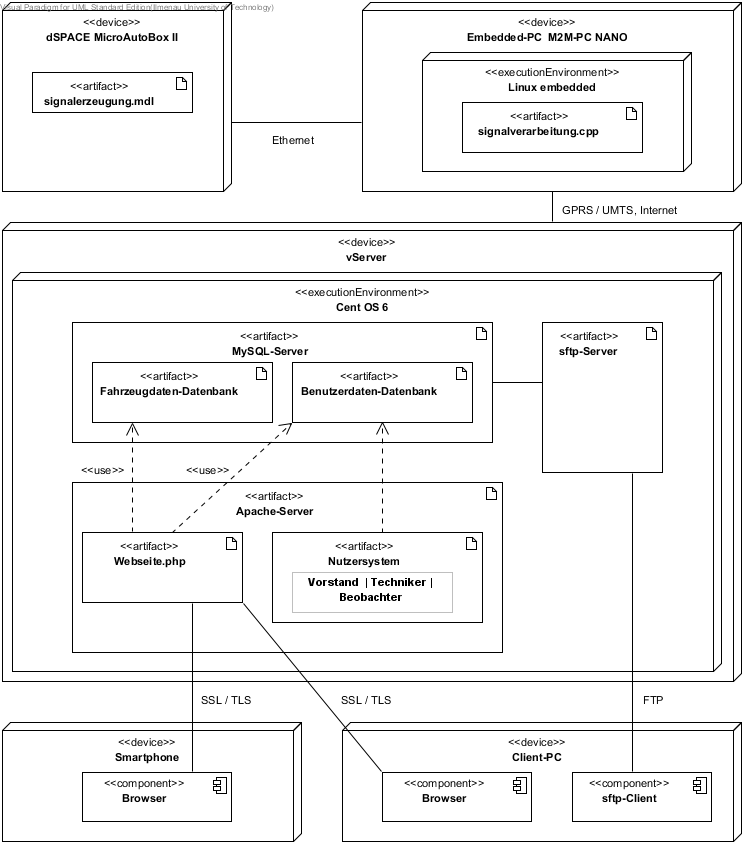
\includegraphics[scale = 0.7]{verteilungsdiagramm.png}
\caption[Verteilungsdiagramm Gesamtsystem]{Gesamtsystem als Verteilungsdiagramm} 

\end{figure}

\subsection{dSPACE MicroAutoBox II}

Bei der dSPACE MicroAutoBox II handelt es sich um ein Steuergerät mit Echtzeiteigenschaften, welches fest im Formula-Student-Fahrzeug verbaut ist und es ermöglicht, sämtliche Fahrzeugdaten aus ebendiesem auszulesen. Auf diesem Gerät wird ein Simulink-Modell implementiert, das die als Busarray empfangen Daten entgegen nimmt, aufbereitet, enkodiert und über eine UDP-Schnittstelle an einen Embedded-PC überträgt. 

\subsection{Embedded-PC}

Die verwendete MicroAutoBox II sendet die zuvor aufbereiteten Fahrzeugwerte mit Hilfe des auf ebendieser implementierten Simulink-Modells per UDP-Sockets über einen kabelgebundenen Netzwerkanschluss (LAN) an den Embedded-PC M2M-PC NANO der Firma Adyna. Die Übertragung der Fahrzeugdaten von dem Embedded-PC zu dem virtuellen Server geschieht ebenfalls über UDP-Sockets. Das Programm läuft eigenständig auf dem Embedded-PC und wird automatisch beim Systemstart ausgeführt. Sobald ein UDP-Paket vollständig empfangen wurde, wird es mit einem Zeitstempel versehen, der die Systemzeit des Embedded-PC zum Zeitpunkt des Hinzufügens beinhaltet, und dient dazu, die Aktualität der Daten bei dem Eintreffen auf dem virtuellen Server festzustellen. Anschließend werden die Daten über eine mobile Breitbandverbindung mittels UDP-Sockets an den virtuellen Server weitergeleitet. Für die eigentliche Übertragung zum virtuellen Server über eine GPRS/UMTS-Verbindung ist ein in der Programmiersprache C++ selbst entwickeltes Programm zuständig.		

\subsection{Virtueller Server}

Der virtuelle Server wird von dem Provider 1\&1 bereitgestellt und ist jederzeit über eine feste IP-Adresse erreichbar. Darauf wird eine in der Programmiersprache C++ entwickelte Software implementiert, die eingehende Pakete an einem bestimmten Port entgegennimmt, deren Nutzdaten dekodiert, validiert und in eine auf dem virtuellen Server laufende MySQL-Datenbank schreibt. 

\subsection{Webseite}

Die Webseite übernimmt im Rahmen dieses Systems die Aufgaben der grafischen Benutzer-oberfläche. Sie besitzt zwei Kernaufgaben: das Darstellen der Fahrzeugdaten, die sich in einer Datenbank auf dem Webserver befinden und das Vermeiden von Zugriffen unbefugter Personen auf eben diese Daten. Dies wird durch ein Benutzersystem erreicht, welches nur ausgewählten Personen den Zugang zu den Informationen der Datenbank ermöglicht und diesen somit die Darstellung oder den Export selbiger Informationen zulässt.

\newpage


\subsection{Datenbanken}

Auf dem virtuellen Server läuft ein MySQL-Server der unserem Projekt zur Verfügung steht. Es werden zwei Datenbanken angelegt um Benutzerdaten und die Fahrzeugdaten aufzunehmen. Zusätzlich wird ein Benutzer mit zugehörigem Passwort eingerichtet, der alle Rechte auf die Datenbanken erhält und so dem Programm den Zugriff auf die Datenbanken zu ermöglichen. Für die Initialisierung der Datenbanken wird ein Skript erstellt.

\subsubsection{Benutzerdaten-Datenbank}

Diese Datenbank bildet die Grundlage für das optionale Benutzersystem, in ihr werden später die Nutzer und ihre zugehörigen Berechtigungen gespeichert. Zudem wird der Zeitpunkt des letzten Logins erfasst, um angemeldete Benutzer automatisch abmelden zu können.

\subsubsection{Fahrzeugdaten-Datenbank}

Diese Datenbank bildet die Schnittstelle zwischen dem C++ - Programm, welches die Fahrzeugdaten aus den UDP-Paketen kontinuierlich entgegennimmt und in die Datenbank speichert, sowie der Webseite, welche die Daten anzeigt. Die Tabelle soll mindestens zehn Stunden an Fahrdaten mit einem Intervall von einer Sekunde aufnehmen (36000 Datensätze), ältere Daten werden aus der Datenbank entfernt. Über die Webseite ist ein Export der Daten im CSV-Format möglich. 


%------------------Feiner Rotz-----------------------------------------

\section{Simulink-Modell}
\subsection{Verwendete Blöcke}

Um den Einstieg in unsere im folgenden aufgeführten Modellausschnitte  zu erleichtern, werden im Verlauf dieses Abschnittes alle zur Erstellung des Simulink-Modells für die dSPACE MicroAutoBox II verwendeten Blöcke vorgestellt und ihre Funktionsweise kurz erläutert. 

\subsubsection{Sources}
\begin{itemize}

\begin{figure}[h]
  \centering
\begin{minipage}[b]{2.5cm}
    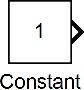
\includegraphics[scale = 0.5]{constant}
    \caption[Constant-Block]{Constant-Block}
  \end{minipage}
\hspace*{3cm}  
  \begin{minipage}[b]{5 cm}
    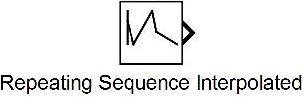
\includegraphics[scale = 0.5]{rsip}
    \caption[Repeating Sequence Interpolated - Block]
    {Repeating Sequence Interpolated - Block}     
  \end{minipage}
\end{figure}

\vspace*{-5mm}

\newpage

\item[1)] \textit{Constant-Block}

Der Constant-Block ermöglicht die Generierung eines reellen oder komplexen, konstanten Wertes. Je nach Modifikation der Einstellungen 
des Blocks wird es zudem ermöglicht, neben einem konstanten Skalar einen konstanten Vektor oder eine konstante Matrix als Eingangssignal bereitzustellen. Als Datentypen für das Eingangssignal stehen die unter A.1 aufgeführten Datentypen zur Verfügung.

\item[2)] \textit{Repeating-Sequence-Interpolated - Block}

Im Gegensatz zum Costant-Block ermöglicht dieser Block die Erzeugung eines individuellen, sich periodisch wiederholenden und kontinuierlichen Signals mittels einer Interpolation anhand zuvor selbst definierter diskreter Zeit- und Funktionswerte, welche in zwei Vektoren gleicher Länge gespeichert sind. 

\end{itemize}

%\newpage

\subsubsection{Ports \& Subsystems}

\begin{itemize}

\begin{figure}[h]
  \centering
  \begin{minipage}[b]{2.5 cm}
    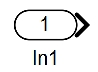
\includegraphics[scale = 0.6]{inport}
    \caption[Inport-Block]{Inport-Block}
  \end{minipage}
  \hfill
  \begin{minipage}[b]{2.5 cm}
    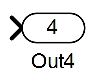
\includegraphics[scale = 0.6]{outport}
    \caption[Outport-Block]{Outport-Block}
  \end{minipage}
  \hfill
  \begin{minipage}[b]{3.5 cm}
    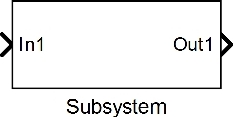
\includegraphics[scale = 0.5]{subsystem}
    \caption[Subsystem]{Subsystem}
  \end{minipage}  
\end{figure}


\item[1)] \textit{Inport-Block}

Dieser Block hat in unserem Modell die Aufgabe, die zuvor festgelegten Eingangssignale des Subsystems auf der Modellebene des Subsystems selbst zu repräsentieren. Darüber hinaus ist es in der Top-Level-Ebene des Systems mit diesem Block auch möglich, externe Eingangssignale aus dem Arbeitsbereich für das Modell bereitzustellen. 

\item[2)] \textit{Outport-Block}

Die Aufgabe des Outport-Blockes ist es, eine Verknüpfung vom aktuellen System zu einem Zielsystem außerhalb der Modellebene herzustellen.

\item[3)] \textit{Subsystem}

Innerhalb eines Subsystems können verschiedene Blöcke zusammengefasst werden, was eine Strukturierung und Gliederung der Signalflüsse erleichtert und zudem eine deutlich übersichtlichere Darstellung des Modells zur Folge hat. Weiterhin ist es auch möglich, mehrere Subsysteme in einem Subsystem zusammenzufassen, um eine beliebige Tiefe innerhalb der Hierarchie eines Modells zu realisieren. \\

\end{itemize}

\newpage

\subsubsection{Signal Routing}

\begin{figure}[h]
\centering
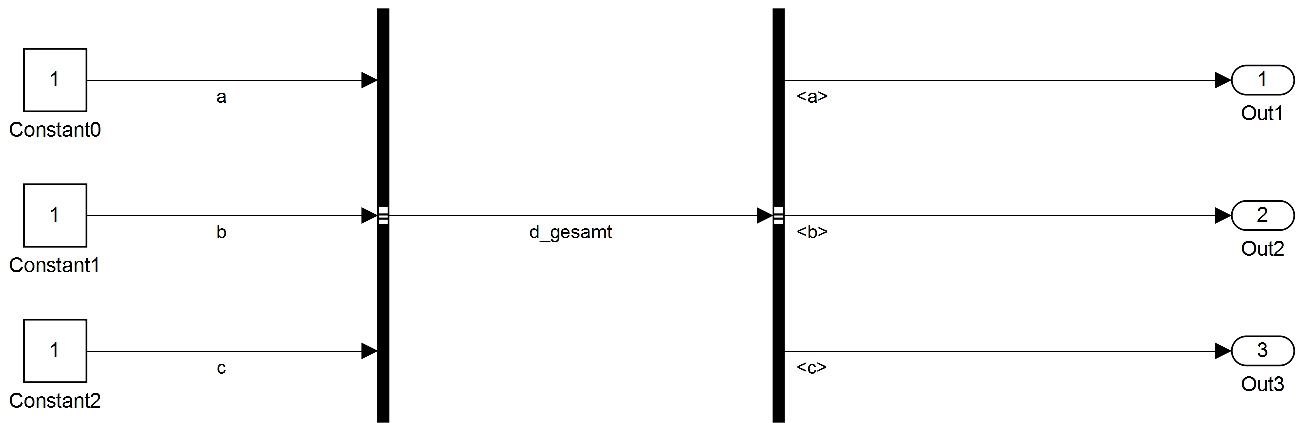
\includegraphics[scale = 0.45]{bus_gesamt}
\caption[Bussystem]
{Bussystem bestehend aus einem Bus Creator (l.) und einem Bus Selector (r.)}
\label{Signal Routing}
\end{figure}


\begin{itemize}

\item[1)] \textit{Bus Creator}

Mit Hilfe eines solchen Bus Creators wird es ermöglicht, mehrere Signale (a, b, c) zu einem Gesamtsignal (d\_gesamt) zu bündeln.

\item[2)] \textit{Bus Selector}

Umgekehrt erlaubt es der Bus Selector, aus einem Gesamtsignal wieder einzelne Signale zu selektieren und diese gesondert weiterzuleiten. So werden wie in Abb. \ref{Signal Routing} dargestellt aus dem Gesamtsignal d\_gesamt wieder die Signale a, b und c herausgeführt. 

\end{itemize}

\subsubsection{Signal Attributes}

\begin{itemize}

\begin{figure}[h]
  \centering
\begin{minipage}[b]{2.5cm}
    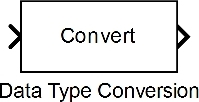
\includegraphics[scale = 0.5]{convert}
    \caption[Convert-Block]{Convert-Block}
    \label{Convert-Block}
  \end{minipage}
\hspace*{3cm}  
  \begin{minipage}[b]{5 cm}
    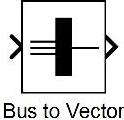
\includegraphics[scale = 0.5]{bustovector}
    \caption[Bus to Vector - Block]{Bus to Vector - Block}
    \label{Bus to Vector - Block}
  \end{minipage}
\end{figure}

\vspace*{-3mm}

\item[1)] \textit{Convert-Block}

Mit dem Convert-Block können verschiedene Anforderungen realisiert werden:

\begin{itemize}
\item Konvertierung eines Signals bzw. eines Signalvektors in einen anderen Datentyp, hierbei kann die Art der Rundung selbst festgelegt werden.

\item Umbenennung eines Signals bzw. eines Signalvektors. \\
Dies hat den Zweck, dass man nach dem Convert-Block unabhängig vom  angelegten Eingangssignal mit einem festen Datentyp und einem fest vergebenem Variablennamen in anderen Systemen bzw. auf anderen Plattformen arbeiten kann.  

\end{itemize} 

\item[2)] \textit{Bus to Vector - Block}

Dieser Block konvertiert ein virtuelles Bussignal in ein Vektorsignal. Hierbei ist es erforderlich, dass alle am zu konvertierenden Bus anliegenden Signale im Datentyp, Signaltyp und im gewählten Sampling-Verfahren übereinstimmen.

\end{itemize}

\subsubsection{Sinks}

\begin{itemize}

\begin{figure}[h]
  \centering
  \begin{minipage}[b]{2.75 cm}
    
\includegraphics[scale = 0.6]{terminator}
    \caption[Terminator-Block]{Terminator-Block}
  \end{minipage}
  \hfill
  \begin{minipage}[b]{2.5 cm}
    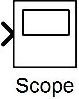
\includegraphics[scale = 0.6]{scope}
    \caption[Scope]{Scope}
  \end{minipage}
  \hfill
  \begin{minipage}[b]{3.5 cm}
    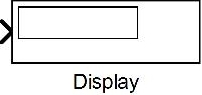
\includegraphics[scale = 0.6]{display}
    \caption[Display]{Display}
  \end{minipage}  
\end{figure}


\item[1)] \textit{Terminator}

Der Terminator dient dazu, die Signale, deren Ausgänge nicht mit Blöcken o.Ä. verbunden sind, abzuschließen. 

\item[2)] \textit{Scope}

Der Scope-Block stellt den Signalverlauf eines Signals über der Simulationszeit dar, weswegen er sich hervorragend dafür eignet, ein erstelltes Modell auf dessen Korrektheit zu überprüfen.

\item[3)] \textit{Display}

Der Display-Block zeigt den konkreten Wert eines Eingangssignals an. Um die Anzeige des Displays anzupassen, kann der Entwickler über die Einstellungen der Format-Parameter Einfluss darauf nehmen. \\ 

\end{itemize}

\subsubsection{Math Operations}

\begin{itemize}

\begin{figure}[h]
\centering
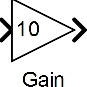
\includegraphics[scale = 0.5]{gain}
\caption[Gain-Block]{Gain-Block zur Verstärkung von Signalen}
\label{Gain-Block}
\end{figure}

\item[1)] \textit{Gain-Block}

Der Gain-Block multipliziert das Eingangssignal mit einer selbst gewählten Konstante, wobei das Eingangssignal selbst ein Skalar, ein Vektor oder eine Matrix sein kann.

\end{itemize}

\newpage

\subsubsection{dSPACE-Blöcke}

Im Folgenden sollen nun diejenigen Blöcke vorgestellt werden, welche speziell für eine Verwendung mit der MicroAutoBox II konzipiert wurden und u. a. für eine Kommunikation ebendieser mit dem Embedded-PC unerlässlich sind. 

\begin{itemize}

\item[1)] \textit{Encode32-Block}

\begin{figure}[h]
\centering
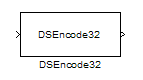
\includegraphics[scale = 1]{dsencode32}
\caption{Block zur Erzeugung eines \textit{uint32}-Datenstroms}
\label{DSEncode32-Block}
\end{figure} 

Der Encoder-Block DSEncode32 basiert auf einer sFunction die von dSPACE implementiert wurde. Diese konvertiert einen Eingangsvektor in einen Datenstrom mit dem Datentyp \textit{uint32}. Dieser Schritt ist notwendig um die Daten für die Übertragung mittels einer UDP-Verbindung vorzubereiten, da die dafür vorgesehenen Blöcke nur Daten dieses Typs übertragen können. 

\item[2)] \textit{UDP-Setup-Block} 

\begin{figure}[h]
\centering
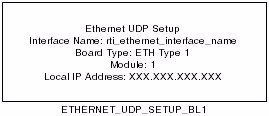
\includegraphics[scale = 1]{ethernet_udp_setup_block}
\caption{UDP-Block zur Einstellung der Netzwerkschnittstelle}
\end{figure}

Der Block ETHERNET\_UDP\_SETUP\_BL1 (\*Abbildung\*) dient zur Initialisierung der Netzwerkschnittstelle. Dort können lokale Portnummern für bis zu 4 Sockets pro Ethernet Interface vergeben und die IP-Adresse sowie Portnummer eines entfernten Geräts (hier: Embedded-PC) konfiguriert werden.

\newpage

\item[3)] \textit{UDP-Send-Block}

\begin{figure}[h]
\centering
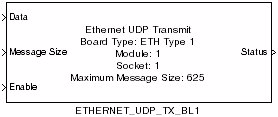
\includegraphics[scale = 1]{ethernet_udp_send_block.png}
\caption{UDP-Block zum Senden eines \textit{uint32}-Datenstroms}
\end{figure}

Das Senden der Daten erfolgt über den Block ETHERNET\_UDP\_TX\_BL1. Diesem wird ein Datenstrom vom Typ \textit{uint32} übergeben, sowie die Größe der zu übermittelnden Daten. Anschließend werden die Daten entsprechend der Konfiguration im ETHERNET\_UDP\_SETUP\_BL1 Block versendet.

\end{itemize}

\subsection{Signalgenerator}

Das Modell, welches auf der dSPACE MicroAutoBox II implementiert wird, besitzt zwei Subsysteme - den Signalgenerator und den Signalkollektor. Der Signalgenerator hat hierbei die Aufgabe, auf der MicroAutoBox II die für einen Systemtest benötigten Testsignale zu generieren, welche anschließend zum Embedded-PC via UDP-Schnittstelle gelangen und daraufhin über eine GPRS/UMTS-Verbindung an einen virtuellen Server gesendet werden. Dieses Subsystem wird jedoch nach einem erfolgreichen Test des Service-Interfaces durch ein Subsystem von Team StarCraft e.V. ersetzt, welches im Stande ist, die im Formula-Student-Fahrzeug verbauten Komponenten anzusprechen und somit im Unterschied zu dem aktuell verwendeten Signalgenerator statt künstlich erzeugter Daten die realen Daten auszulesen und an den Signalkollektor weiterzuleiten. \vspace*{5mm}

\begin{figure}[h]
\centering
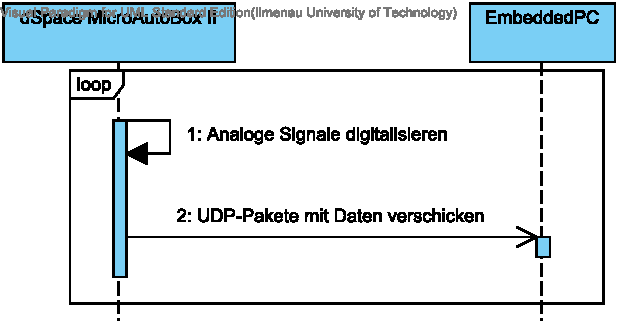
\includegraphics[scale = 1]{opt_autobox}
\caption[Sequenzdiagramm Simulink-Modell]
{Sequenzdiagramm des auf der MicroAutoBox II implementierten Simulink-Modells}
\end{figure}

\newpage

\subsubsection{Struktur des Subsystems}

Um ein hohes Maß an Übersichtlichkeit und Modularität zu gewährleisten, wird an den Vorgaben von Team StarCraft e.V. orientierend das Subsystem des Signalgenerators nochmals in einzelne Subsysteme unterteilt, die die verschieden Kategorien der jeweiligen Fahrzeugdaten repräsentieren (s. Abb. \ref{Subsysteme}): \\

\begin{figure}[h]
\centering
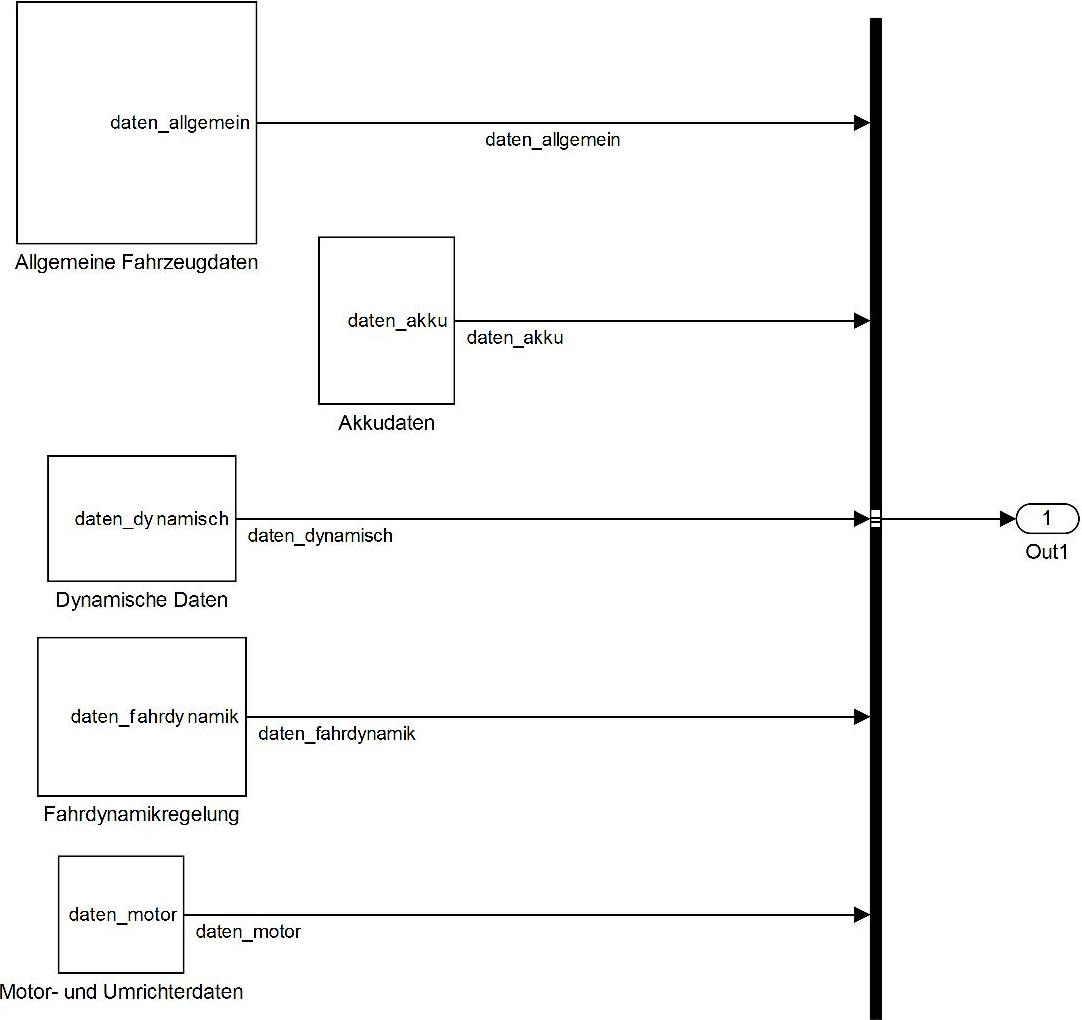
\includegraphics[scale = 0.85]{signalgen}
\caption[Subsysteme des Signalgenerators]
{Subsysteme des Signalgenerators nach den Kategorien der Fahrzeugdaten}
\label{Subsysteme}
\end{figure}

\newpage

\begin{figure}[h]
\centering
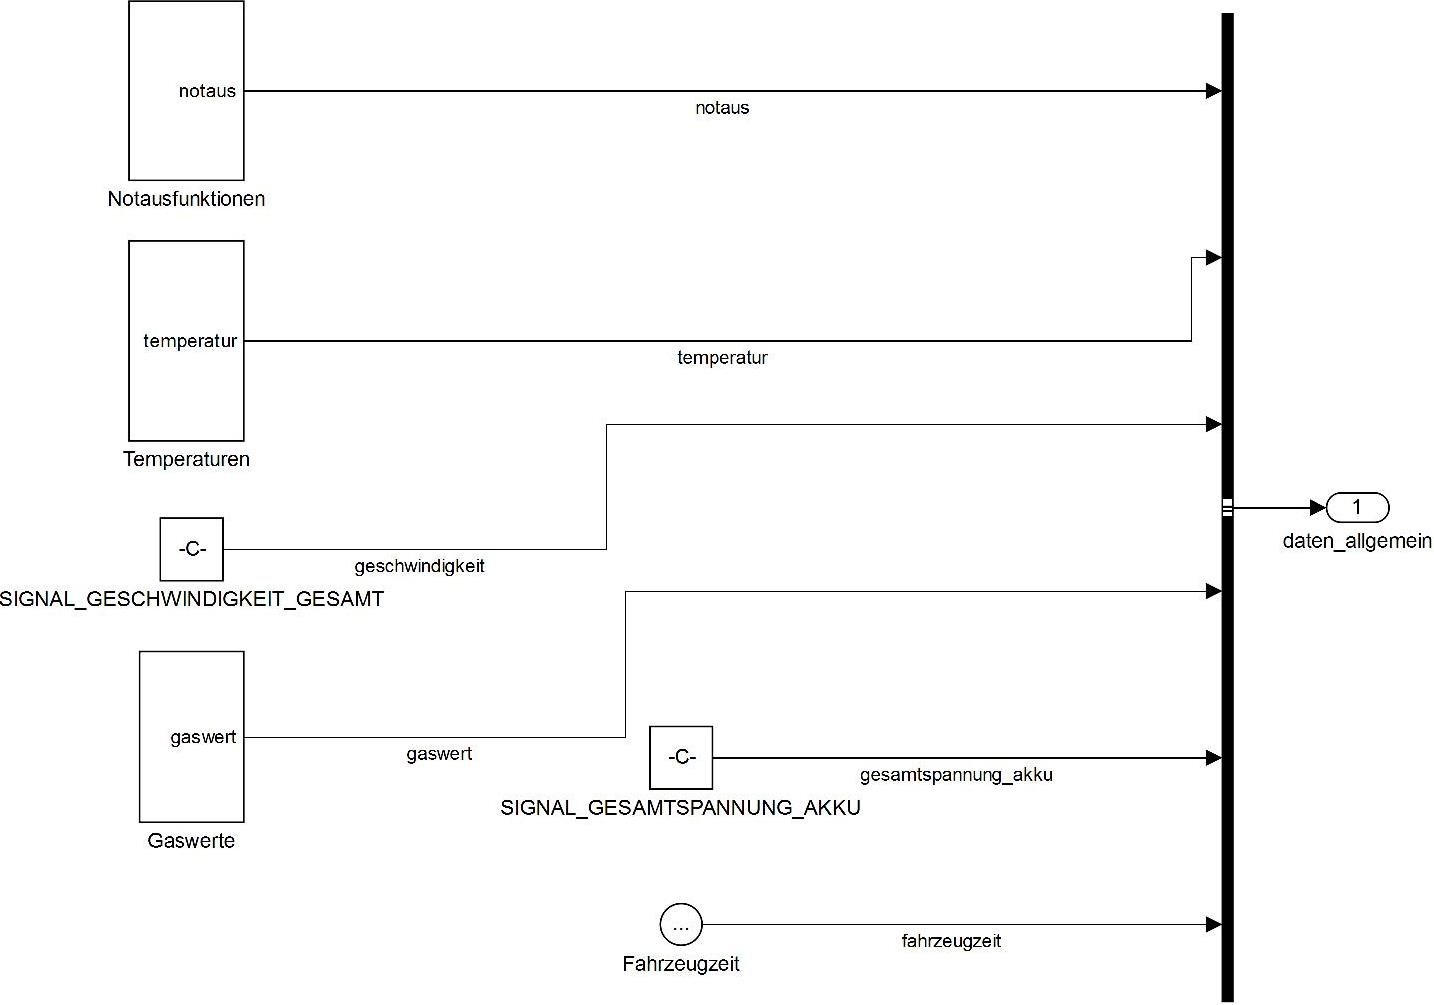
\includegraphics[scale = 0.65]{suballgemein}
\caption[Subsystem "`Allgemeine Daten" des Signalgenerators]{Subsystem "`Allgemeine Daten"\ des Signalgenerators}
\label{Signalgenerator}
\end{figure}

Innerhalb dieser Subsysteme findet nun - ohne Beschränkung der Allgemeinheit am Subsystem "`Daten Allgemein"\ erläutert - die Signalerzeugung (Geschwindigkeit, Gesamtspannung des Akkus und der Fahrzeugzeit) statt, wobei wie in Abbildung \ref{Signalgenerator} dargestellt die Signalerzeugung mehrere Signale der gleichen "`Signalgruppe"\ wiederum zu Subsystemen (Notausfunktionen, Temperaturen und Gaswerte)  innerhalb des Subsystems "`Allgemeine Daten"\ zusammengefasst werden. Die eigentliche Erzeugung der Signale wird wie in Abbildung \ref{Signalerzeugung_temp} gezeigt mittels Blöcken aus der Kategorie "`Sources" (s. Seite 8) realisiert. Hierbei wird je nach Input entweder ein Constant-Block mit dem Datentyp \textit{boolean} zur Realisierung von Schaltern etc. (s. Notausfunktionen) oder ein Repeating Sequence Interpolated (RSI) - Block mit dem Datentyp \textit{single} zur Modellierung der restlichen Fahrzeugkomponenten verwendet (s. Gaswerte). Der Datentyp \textit{single} wurde deshalb gewählt, um auch wie von Team StarCraft e.V. gefordert als Input Werte mit mehreren Nachkommastellen realisieren zu können. Die auf analoge Weise in Abbildung \ref{Signalerzeugung_temp} mit Constant- oder RSI-Blöcken erzeugten 386 Input-Signale werden schließlich im Umkehrschluss zur obigen Beschreibung über mehrere Bussysteme und Subsysteme zu einem Busarray im Signalgenerator zusammengefasst, welcher nunmehr dieses an den Signalkollektor übergibt.   

\newpage

  
\begin{figure}[h]
\centering
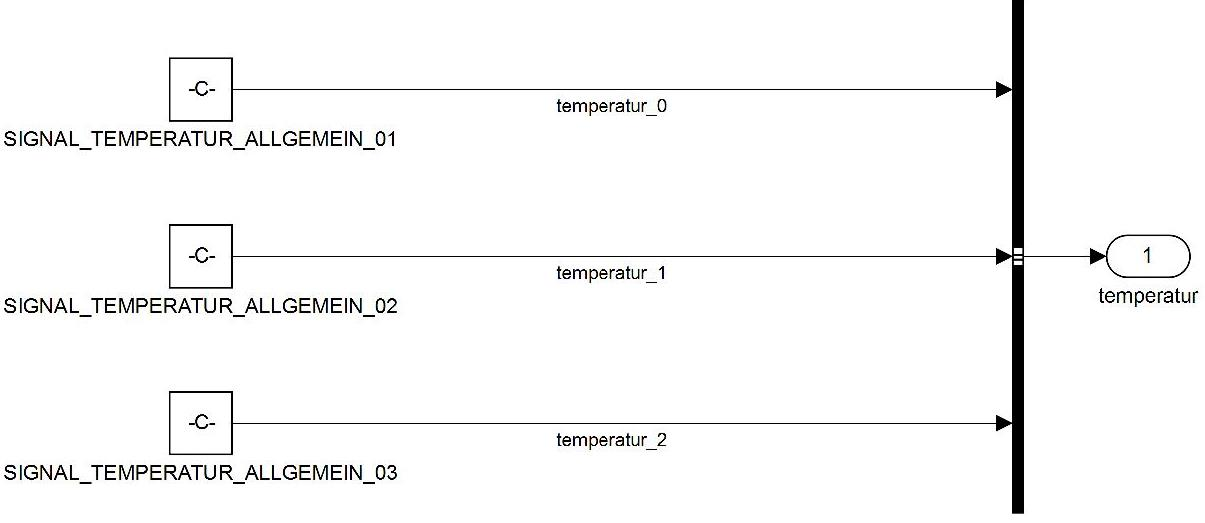
\includegraphics[scale = 0.65]{subsubtemp}
\caption[Subsystem "`Temperaturen" \ ]{Signalerzeugung im Subsystem "'Temperaturen" \ }
\label{Signalerzeugung_temp}
\end{figure}

\subsubsection{Config-Datei "`signalgenerator\_microautobox.m" }

Um eine mögliche Änderung der Testsignale zu vereinfachen und eine übersichtliche Darstellung aller Testsignale zu realisieren, sorgt eine Konfigurationsdatei in Matlab für die Spezifizierung der Testsignale des Simulink-Modells. Die in dem *.m-File aufgeführten Parameter für die Zeit- und Funktionsvektoren dienen als Referenz für die signalerzeugenden Blöcke, welche über den Workspace von Matlab auf diese nach dem Ausführen der Datei zugreifen können (s. Abb. \ref{Ref. RSI}). Hierbei sollte jedoch beachtet werden, dass vor dem Kompilieren des Simulink-Modells und der Implementierung ebendiesem auf der MicroAutoBox II einmalig das *.m-File ausgeführt werden muss. Demzufolge muss auch nach dem Ändern von Parametern die Datei neu ausgeführt werden, damit bei einer erneuten Implementierung des Simulink-Modells die geänderten Parameter korrekt übernommen werden können. Zudem wurde jeder Funktionsvektor mit dem Präfix "`SIGNAL\_"\ und jeder Zeitvektor mit dem Präfix "`TIME\_"\ versehen, um die Benennung der Parameter im *.m-File zu standardisieren. \\

\begin{figure}[h]
\centering
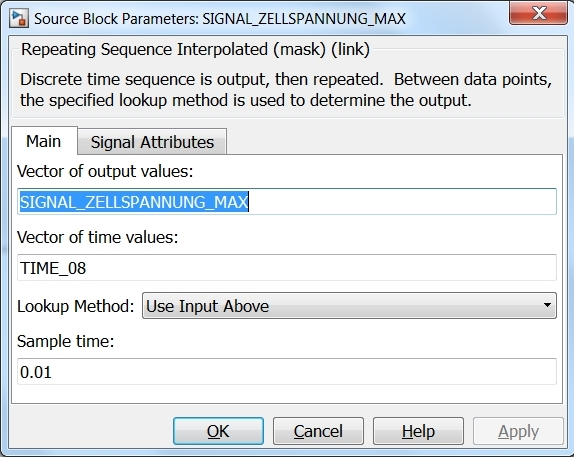
\includegraphics[scale = 0.55]{referenz}
\caption[Referenzierung der Config-Datei]{Referenzierung im RSI-Block}
\label{Ref. RSI}
\end{figure}

\newpage

\subsection{Signalkollektor}

Der Signalkollektor stellt wie bereits erwähnt das zweite große Subsystem innerhalb des Simulink-Modells dar. Er hat die Aufgabe, den vom Subsystem "`Signalgenerator"\ (s. 3.2.2) oder von einem späteren Subsystem von Team StarCraft e.V. erhaltenen Busarray wieder in die einzelnen Signale zu unterteilen, ggf. geeignet aufzubereiten und diese dann an eine UDP-Schnittstelle innerhalb des Subsystems weiterzuleiten, welche die erzeugten Testsignale bzw. Testdaten an den Embedded-PC sendet.  

\subsubsection{Struktur des Subsystems}

Das Subsystem selbst besitzt die folgende innere Struktur: \\
In einem ersten Schritt wird das Busarray wieder in den Kategorien A) - E) der Fahrzeugdaten entsprechenden Signalgruppen aufgeteilt und den fünf Subsystemen (analog zu Abb. \ref{Subsysteme}) zugeführt. Dort werden die nunmehr fünf Busarrays wieder über mehrere Busselektoren und Subsysteme hinweg in die 368 einzelnen Signale aufgelöst, welche somit einzeln aufbereitet werden können (s. Abb. \ref{Signalaufbereitung_allg}). \\

\begin{figure}[h]
\centering
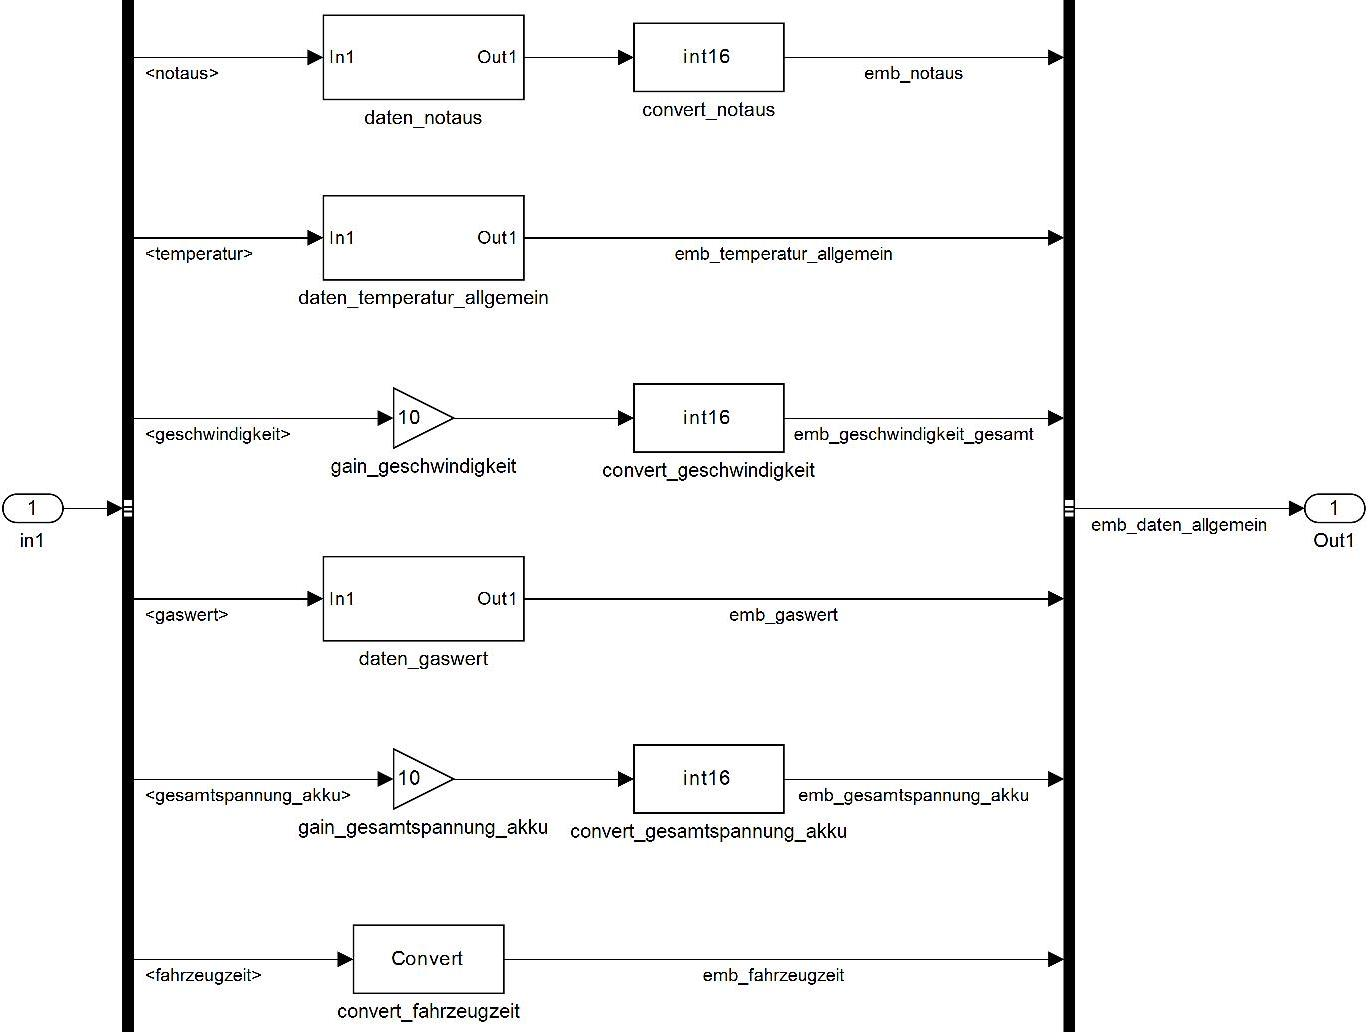
\includegraphics[scale = 0.70]{collallgemein}
\caption[Signalaufbereitung im Subsystem "`daten\_allgemein" \ ]{Signalaufbereitung im Subsystem "`daten\_allgemein" \ }
\label{Signalaufbereitung_allg}
\end{figure} 

\newpage


Während der Aufbereitung der Signale werden die folgenden Schritte durchgeführt:

\begin{itemize}

\item[1)] \textit{Verstärkung der Signale}

Abhängig von der Anzahl der Nachkommastellen des Testsignals $n\ mit\ n>0$ wird dieses nun durch einen Gain-Block (s. Abb. \ref{Gain-Block}) mit dem Faktor $10^n$ multipliziert, um für den aktuellen Wert des Testsignals jeweils einen ganzzahligen Wert zu erhalten, was zur Vereinheitlichung der zu übertragenden Daten beiträgt.

\item[2)] \textit{Konvertierung der Datentypen}

Die nunmehr ganzzahligen Werte werden von ihren Datentypen \textit{boolean} oder \textit{single} nun einheitlich mittels eines Convert-Blocks (s. Abb. \ref{Convert-Block}) in den Datentyp \textit{int16} konvertiert, wodurch alle Signale den gleichen Datentyp aufweisen.  

\item[3)] \textit{Umbenennung der Variablennamen}

Mit dem Convert-Block ist es zudem möglich, dem Ausgangssignal unabhängig vom Eingangssignal einen festen bzw. neuen Variablennamen zu vergeben. Dies ist insofern nützlich, da bei einem möglichen Zugriff auf die Daten bzw. die Variablen durch den Embedded-PC diese immer die gleichen Variablennamen besitzen, unabhängig davon ob der Signalgenerator durch das Subsystem von Team StarCraft e.V. ersetzt wurde oder nicht.

\end{itemize}  

Nachdem die Daten anhand der obigen Schritte aufbereitet wurden, werden diese erneut durch mehrere Bus Creator und Subsysteme auf einem zentralen Bus Creator zu einem Busarray gebündelt und auf einen Bus to Vector - Block (s. Abb. \ref{Bus to Vector - Block}) gegeben, welcher das Busarray in einen Vektor umwandelt. Anschließend wird dieser Vektor einem Encoder (s. Abb. \ref{DSEncode32-Block}) zugeführt.

\subsection{Enkodierung}

Die Enkodierung der Signale erfolgt in einem DSEncode32-Block von dSPACE (s. Seite 12). Dort werden die Signale so aufbereitet, dass sie über eine UDP-Schnittstelle übertragen werden können. 

\subsection{UDP-Schnittstelle} 

Die UDP-Schnittstelle wird mithilfe zweier Simulink-Blöcke realisiert (s. Seite 12). 

\newpage

\section{Embedded-PC}

\begin{figure}[h]
\centering
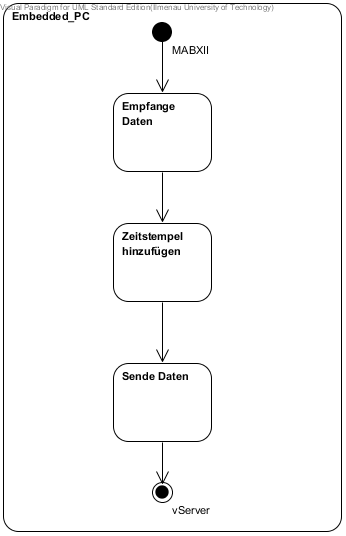
\includegraphics[scale = 0.70]{activity_embedded_pc.png}
\caption[Aktivitätsdiagramm Embedded-PC]{Aktivitätsdiagramm des Embedded-PCs}
\end{figure} 

\subsection{Empfangen der Fahrzeugdaten}

Der Embedded-PC lauscht an einem fest definierten Port nach Paketen, welche zuvor von der MicroAutoBox II über eine Ethernet-Vebindung verschickt wurden. Die Übertragung erfolgt mittels des verbindungslosen Netzwerkprotokolls UDP und wird mithilfe von Unix Domain Sockets (SOCK\_DGRAM) realisiert. 

\subsection{Hinzufügen eines Zeitstempels}

Da es nicht ausgeschlossen ist, dass sich Pakete bei der Übertragung überholen und/oder aufgrund einer schlechten Verbindung erst sehr spät das Ziel erreichen, erhält ein Paket sobald es entgegengenommen wird einen Zeitstempel um im späteren Verlauf veraltete Pakete identifizieren zu können. 

\subsection{Senden der Fahrzeugdaten}

Im Embedded-PC werden die Daten - bis auf das Hinzufügen eines Zeitstempels - nicht verändert. Sie werden also lediglich durchgereicht und mittels Unix Domain Sockets (SOCK\_DGRAM) an den virtuellen Server über eine GPRS/UMTS-Verbindung übertragen. 

\section{Virtueller Server}

Im Folgenden wird die Funktionsweise des virtuellen Servers anhand eines Aktivitäts-Diagrammes modelliert. Innerhalb des Programmes werden die Paketdaten in einem Datenobjekt gespeichert, in dem bereits grundlegende Funktionen (z.B. Abfrage des Embedded-PC-Zeitstempels) implementiert sind. Das Objekt wird in den einzelnen Schritten so aufbereitet, dass es letztendlich in die Datenbank geschrieben werden kann. Zur besseren Fehlerbehandlung in der Implementierungs- und Testphase wird eine Logging-Klasse eingerichtet. Diese wird im fertigen Programm nicht mehr zur Verfügung stehen, die Aktivierung erfolgt während der Kompilierung über Makros. \\

\begin{figure}[h]
\centering
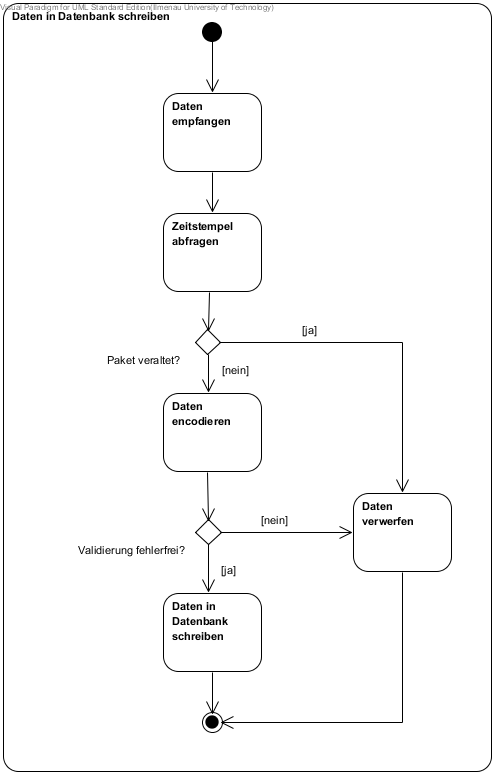
\includegraphics[scale = 0.70]{activity_vserver.png}
\caption[Aktivitätsdiagramm vServer]{Aktivitätsdiagramm des virtuellen Servers}
\end{figure}

\newpage


\subsection{Empfangen der Fahrzeugdaten}

Durch die starke Ähnlichkeit in der Funktionsweise mit 3.3.1 werden sich diese Abschnitte große, wenn nicht sogar alle Teile der Implementation teilen. Diese Maßnahme soll nicht nur dazu führen, dass Fehler in der Programmierung und Konzipierung reduziert werden, sondern auch, dass zusätzlicher Zeitaufwand vermieden wird. 

\subsection{Abfragen des Zeitstempels}

Hier wird der in 3.3.2 hinzugefügte Zeitstempel abgefragt. Um veraltete Pakete identifizieren zu können wird in einer Variable der aktuellste Zeitstempel zwischengespeichert und mit allen ankommenden Paketen verglichen. Pakete, die zu alt sind (ein genauer Wert hierfür muss bei praktischen Versuchen ermittelt werden) werden verworfen. 

\subsection{Daten dekodieren}

Die in 3.2.4 enkodierten Daten werden in diesem Schritt wieder dekodiert und so aufbereitet, dass sie in die Datenbank geschrieben werden können. Der Algorithmus zur Dekodierung kann aus einer von dSPACE erstellten sFunction (C Code) DSDecode32 ermittelt werden. Treten beim Dekodiervorgang keine Fehler auf, gehen wir davon aus, dass das Paket korrekt übertragen wurde und führen bis auf das Prüfen der Wertebereiche keine weitere Fehlerkontrolle durch. Falls Fehler auftreten, wird das Paket verworfen und eine Fehlermeldung in den entsprechenden Eintrag in der Datenbank geschrieben. Eine Fehlerkorrektur findet nicht statt. Die Daten liegen anschließend in einem Vektor bestehend aus \textit{int16}-Werten vor. 

\subsection{Daten verwerfen}

Daten, die veraltet sind oder nicht dekodiert werden konnten, werden verworfen. 

\subsection{Daten in Datenbank schreiben}

Die Anfragen an die MySQL-Datenbank erfolgen mittels des MySQL Connector/C++. Dabei handelt es sich um eine C++ API die es erlaubt mittels TCP- oder UNIX-Sockets die Verbindung zu einer MySQL-Datenbank herzustellen und Anfragen zu übergeben. 

\newpage

\section{Webseite}

Anhand des nachfolgenden Diagramms soll das Verhalten der Webseite exemplarisch dargestellt werden. Ein registrierter Benutzer ruft in einem Webbrowser die Seite des Service Interfaces auf und loggt sich anschließend über das ihm angezeigte Formular im System ein. Anschließend wird er auf die Seite der allgemeinen Fahrzeugdaten weitergeleitet. Über das Menü steht ihm die Auswahl frei, sich die nach unterschiedlichen Kategorien sortierten Fahrzeugdaten anzeigen zu lassen. Am Beispiel der Akkudaten ruft der Nutzer im Menü über einen Klick auf den Reiter "`Akkudaten"\ die Seite akkudaten.php auf. Dieses PHP-Skript öffnet eine MySQL-Verbindung und führt nach einem erfolgreichen Verbindungsaufbau eine MySQL-Anfrage aus, die die aktuellsten Akkudaten aus der Fahrzeugdatenbank ermittelt und schließt die Verbindung anschließend wieder. Diese ermittelten Daten werden nun auf unterschiedlichster Art und Weise auf der Webseite dargestellt, sei es nun z.B. als Tabelle oder als einzeln hervorgehobene und gekennzeichnete Sonderinformationen.
Ein JavaScript, welches gleichzeitig im Hintergrund läuft, sorgt dafür, dass die Daten alle $1000 ms$ aktualisiert werden ohne die komplette Seite vollständig neu zu laden. Dabei - und unter Berufung auf die weichen Echtzeitanforderungen - wird die Aktualisierung mittels Timeout realisiert. Anstelle den Server alle $1000 ms$ aufzufordern neue Daten zu schicken, wird nach dem Erhalt der Daten $1000 ms$ gewartet bis eine neue Anfrage gestartet wird. Dies hat zum Vorteil, dass der Server nicht unnötig belastet wird.
Der Benutzer hat jederzeit die Möglichkeit durch die Auswahl eines anderen Reiters im Menü, sich andere Fahrzeugdaten darstellen zu lassen. Das Verhalten läuft analog ab. Vor dem Verlassen wird der Benutzer angehalten sich auszuloggen und seine aktuelle Sitzung somit zu beenden. \\



\begin{figure}[h]
\centering
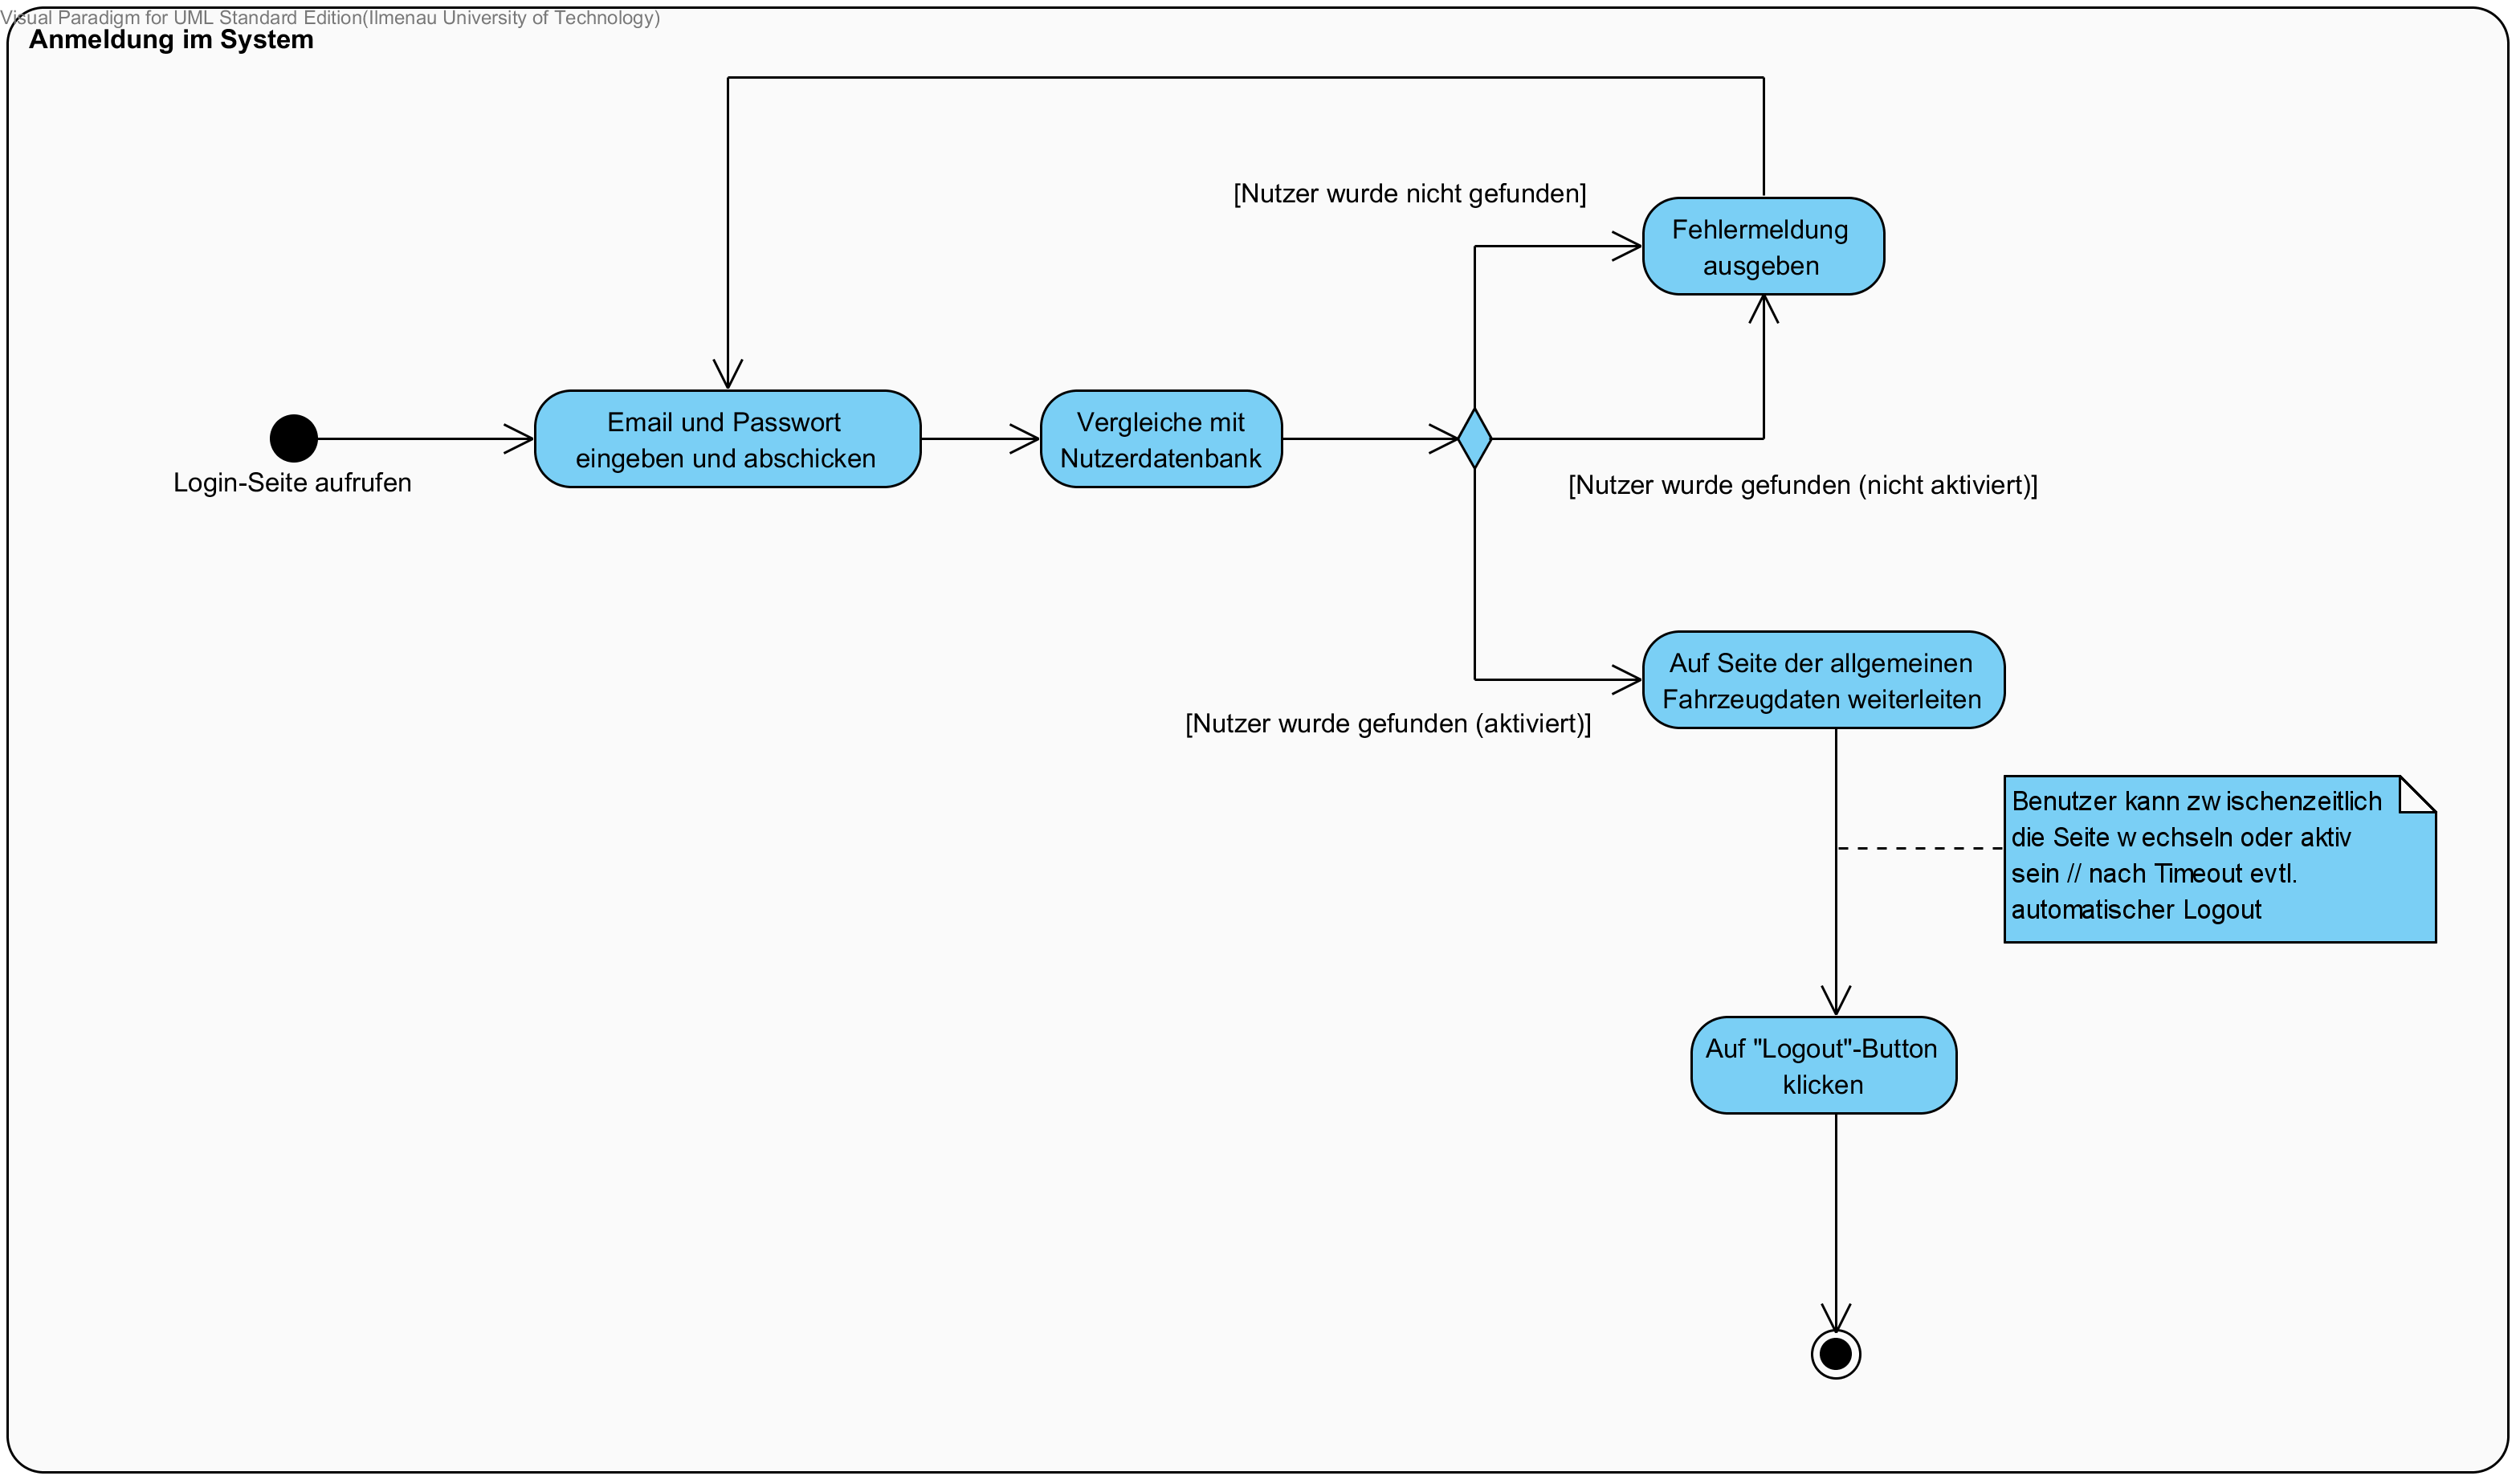
\includegraphics[scale = 0.6]{anmeldungsvorgang}
\caption[Aktivitätsdiagramm Anmeldevorgang]{Aktivitätsdiagramm des Anmeldevorgangs}
\label{Anmeldevorgang}
\end{figure}

\newpage

\subsection{Registrierung}

Durch das Aufrufen der Seite des TeamStarcraft e. V. Teams lässt sich das Service Interface für das Formula Student Fahrzeug erreichen. Der Besucher erhält eine Aufforderung sich einzuloggen. Es können hierbei unterschiedliche Fälle eintreten (s. Abb. \ref{Anmeldevorgang}): 

\begin{itemize}

\item \textit{Fall 1: Der Besucher ist noch nicht registriert.} \\
Sollte er sich noch nicht registriert haben, kann er dies über einen Klick auf einen "`Hier registrieren"\ - Button tun. Der Besucher wird auf eine neue Seite weitergeleitet, die ihm mehrere Formularfelder zur Verfügung stellt. Neben dem Namen (Vor- und Nachname) wird er noch aufgefordert seine E-Mail-Adresse und ein Password eingeben. Das eingegebene Passwort muss aus mindestens 6 Zeichen (erlaubt sind Buchstaben in Groß- und /oder Kleinschreibung sowie Ziffern und Sonderzeichen, wobei von jeder Sorte mindestens eines enthalten sein muss) bestehen und muss einmal wiederholt werden. Anschließend kann der Besucher das Anmeldeformular durch einen Klick auf einen Button abschicken. Entsprechen alle Eingaben den Vorgaben werden die Formulardaten in die Nutzerdatenbank eingetragen, andernfalls wird der Nutzer aufgefordert sich mit anderen Daten zu registrieren. Dabei wird das Passwort in verschlüsselter Form und nicht im Klartext abgespeichert. Es wird zudem der Status des Benutzers auf "`nicht aktiviert"\ gesetzt. Anschließend wird eine E-Mail an den Vorstand generiert, die ihn auf die neue Registrierung im System hinweist. Der Vorstand erhält die Möglichkeit die Daten (mit Ausnahme des Passwortes) der registrierten Nutzer einzusehen und deren Status von "`nicht aktiviert"\ auf "`aktiviert"\ zu setzen oder einzelne Benutzer aus dem System zu löschen. Im Falle der Aktivierung des Accounts generiert das System eine E-Mail, die es an die eingetragene E-Mail-Adresse versendet und den Nutzer über die erfolgreiche Aktivierung seines Accounts hinweist.

\end{itemize}

\subsection{Anmeldung}

\begin{itemize}

\item \textit{Fall 2: Der Benutzer ist bereits angemeldet.} \\ 
Zum Anmelden im System ruft der Nutzer die Login-Seite auf und wird anschließend aufgefordert seine E-Mail-Adresse und sein Passwort einzugeben. Durch einen Klick auf den Login-Button werden die eingegebenen Daten mit der Nutzerdatenbank verglichen. Sollte die Konstellation aus E-Mail-Adresse und dazugehörigem Passwort in der Nutzerdatenbank nicht entdeckt werden, gibt das System eine Fehlermeldung aus, die den Nutzer darauf hinweist, dass die von ihm eingegebenen Daten inkorrekt sind. Sollte das System hingegen einen passenden Eintrag finden, wird abhängig davon, ob der Nutzer bereits aktiviert ist, entweder eine Fehlermeldung (Fall "`nicht aktiviert") ausgegeben, oder der Nutzer auf die Seite der allgemeinen Fahrzeugdaten weitergeleitet (Fall "`aktiviert"). Der Nutzer kann nun auf der Seite nach Belieben, aber unter Berücksichtung der ihm gegebenen Rechte, auf der Seite des Service Interfaces navigieren.
Sollte in einer gewissen Zeitspanne keine Aktivität vom Benutzer erkannt werden, wird er automatisch aus dem System ausgeloggt.
Ansonsten steht ihm die Möglichkeit nach getaner Arbeit offen, sich über den "`Logout"\ - Button auszuloggen und die Seite zu verlassen.

\end{itemize}

\newpage

\subsection{Passwort vergessen}

\begin{figure}
\centering
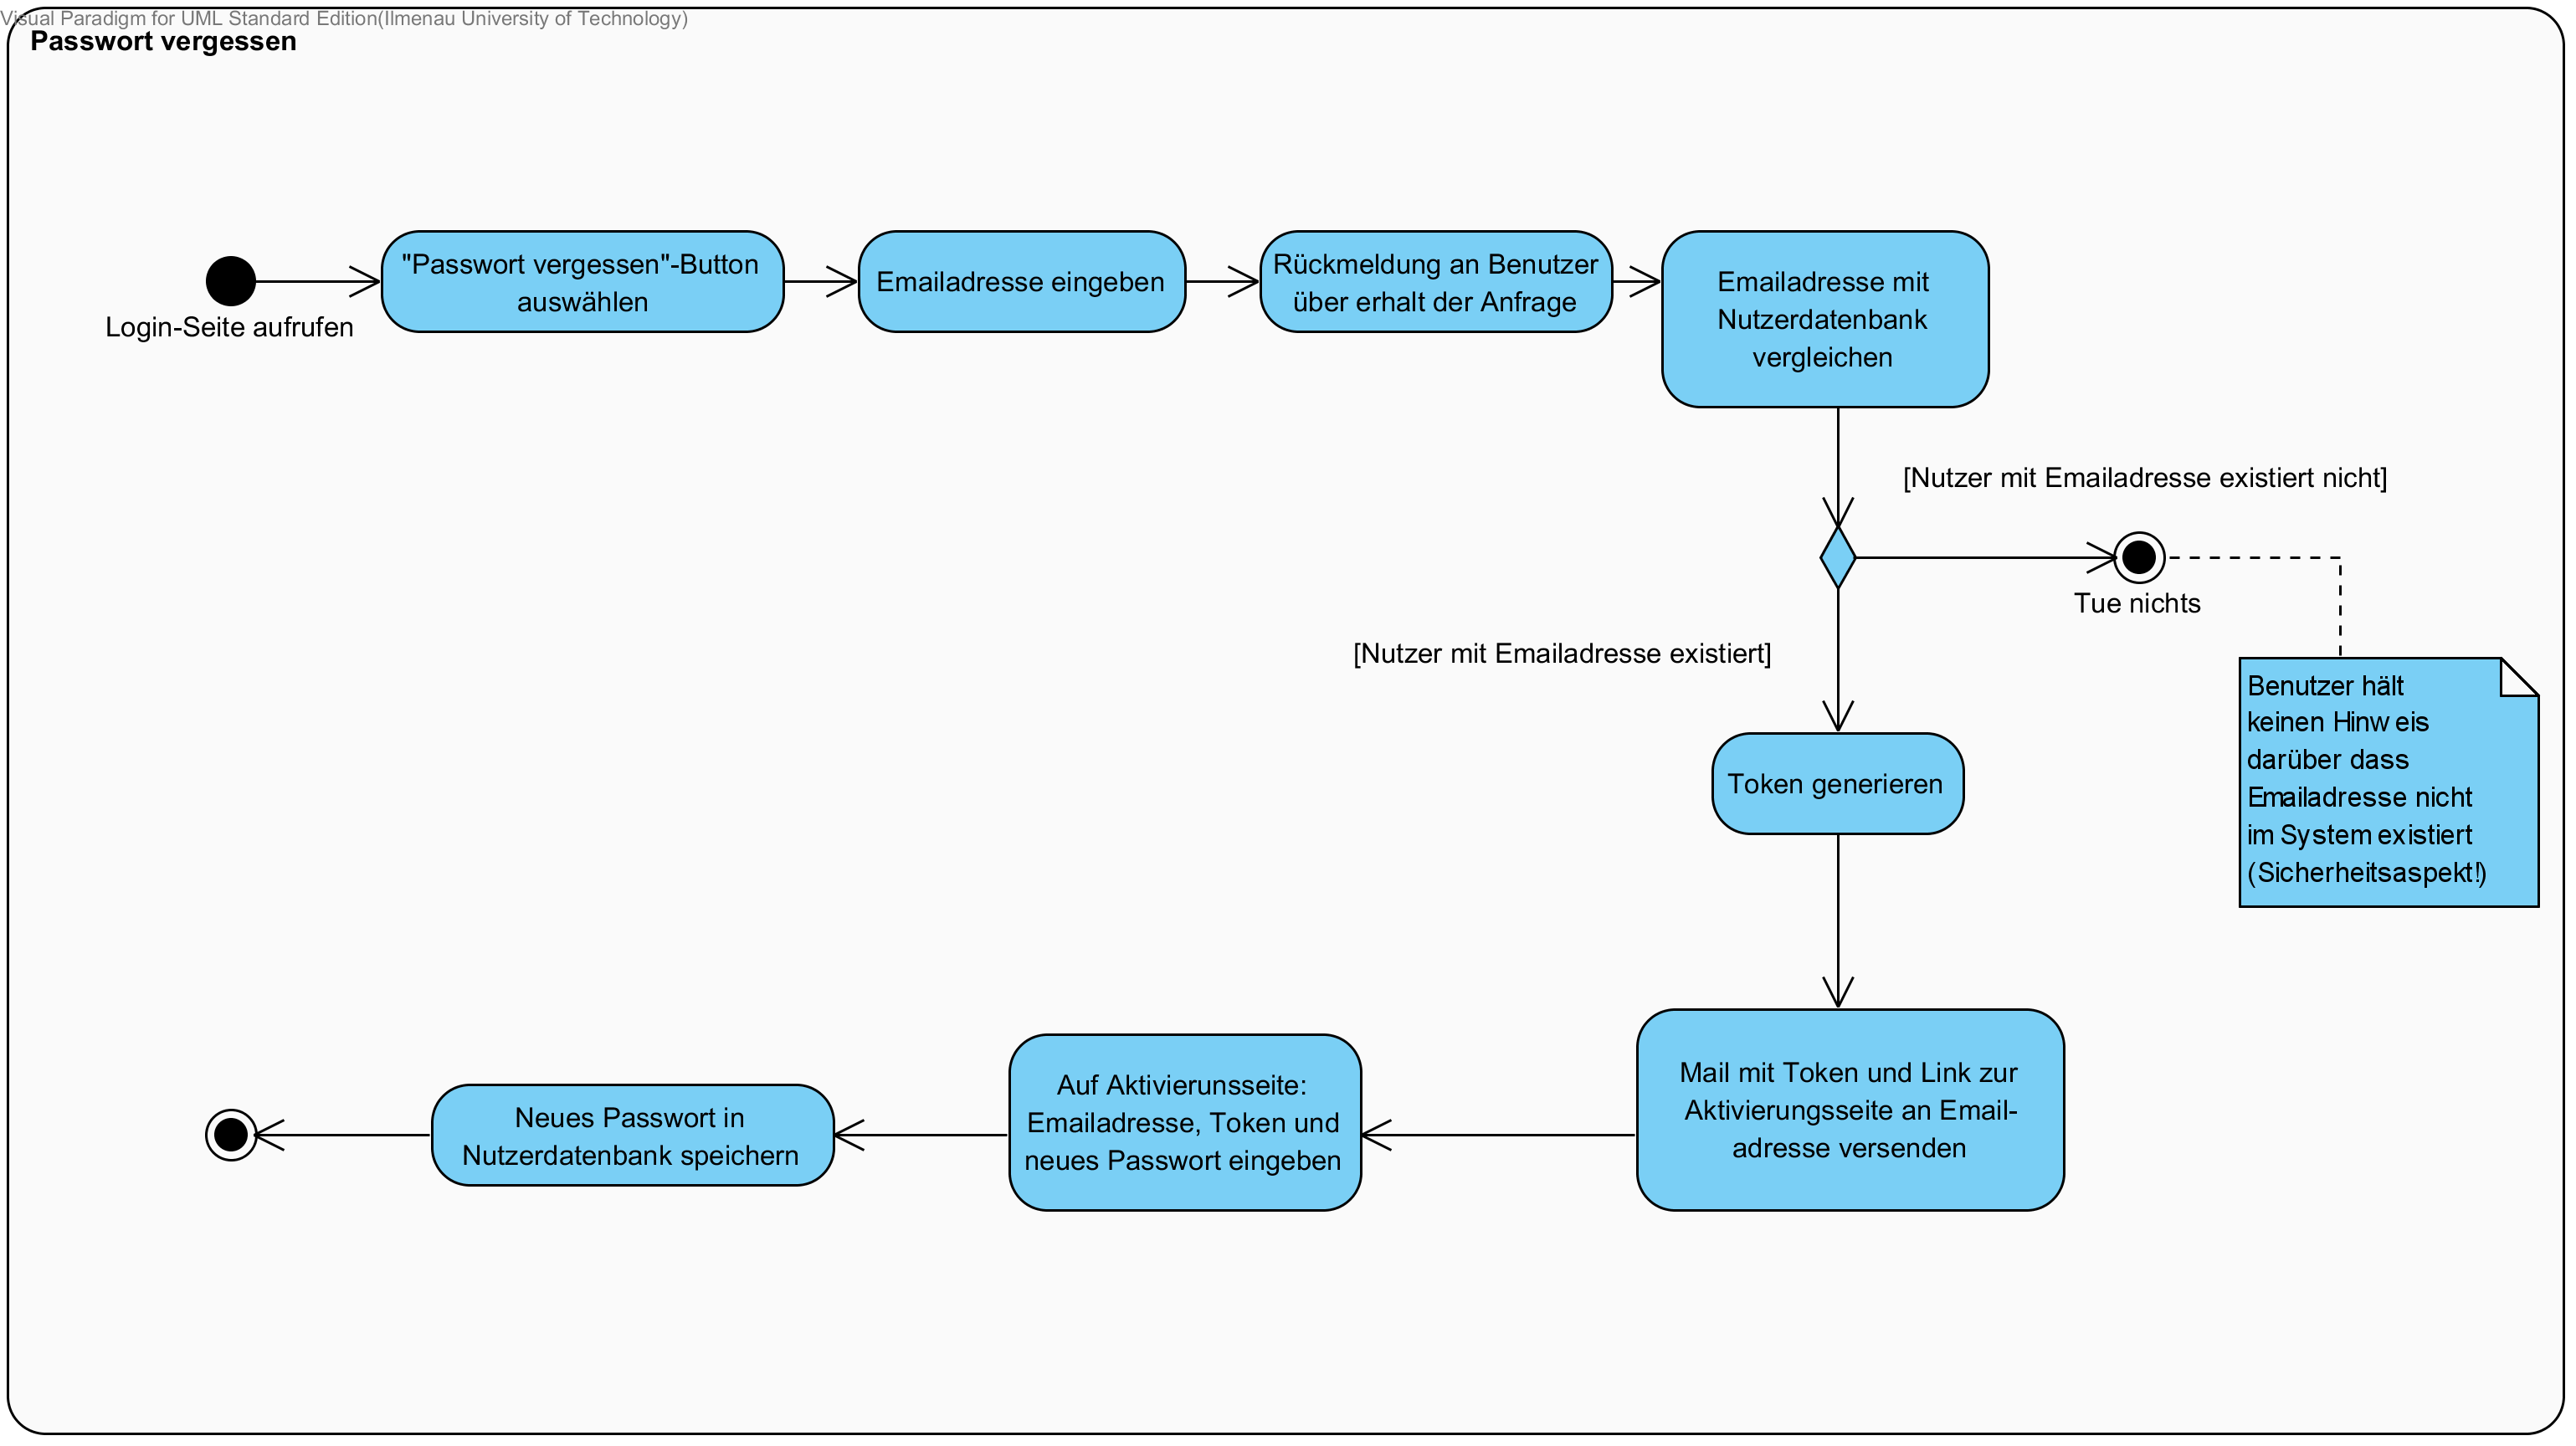
\includegraphics[scale = 0.6]{passwort_vergessen_vorgang}
\caption[Aktivitätsdiagramm Passwort vergessen - Vorgang] {Aktivitätsdiagramm des "`Passwort vergessen"\ - Vorgangs}
\end{figure} 

\begin{itemize}

\item \textit{Fall 3: Passwort vergessen} \\
Tritt der Fall ein, dass ein im System registrierter Benutzer sein Passwort vergisst, bietet das Nutzersystem ihm die Möglichkeit, sich ein neues Passwort zu setzen. Nach dem Aufruf der Login-Seite muss der Nutzer hierfür auf den Button "`Passwort vergessen"\ klicken und wird anschließend auf eine Seite weitergeleitet, die ihn auffordert seine E-Mail-Adresse einzugeben. Durch die Bestätigung der E-Mail-Adresse durch den Benutzer prüft das Nutzersystem im Hintergrund, ob ein Eintrag zu dieser E-Mail-Adresse existiert. Falls nicht, wird der Vorgang abgebrochen. Der Benutzer erhält aus Sicherheitsgründen kein Feedback darüber. Sollte ein entsprechender Nutzer existieren, generiert das System einen Token, den es mitsamt eines Aktivierungslinks an die angegebene E-Mail-Adresse verschickt. Auf der Aktivierungsseite wird der Nutzer erneut aufgefordert seine E-Mail-Adresse und den Token anzugeben. Des Weiteren kann er sich an dieser Stelle ein neues Passwort auswählen (selbe Bedingungen wie bei der erstmaligen Registrierung), welches anschließend das alte Passwort im System überschreibt.

\end{itemize}

\newpage

\subsection{Benutzerverwaltung}

Der Vorstand besitzt als einziger Nutzer im System die Möglichkeit der Verwaltung aller registrierten Systemnutzer. Hierfür steht ihm neben den Übersichtsseiten für die einzelnen Kategorien an Informationen eine spezielle Seite "`Benutzerverwaltung"\ zur Verfügung. Diese Seite stellt die Daten aller angemeldeten Nutzer dar und gibt Auskunft über deren Status im System, also ob sie bereits aktiviert worden sind oder eine Aktivierung noch aussteht. Gelöschte Benutzer werden nicht angezeigt. Ein Aufruf der Seite der Benutzerverwaltung resultiert in einem Verbindungsaufbau mit der Nutzerdatenbank. Bei erfolgreichem Verbindungsaufbau erfolgt anschließend das Versenden eines MySQL-Query, das als Resultat alle im System befindlichen Nutzer ausgibt. Anschließend wird die MySQL-Verbindung wieder getrennt. Die Ausgabe beinhaltet dabei Informationen wie Vor- und Nachname, Rechtegruppe, Accountstatus und eine Information über den letzten Zeitpunkt einer Aktivität des Nutzers. Mittels verschiedener Buttons erhält der Vorstand die Möglichkeit alle Nutzer komplett zu verwalten, d.h. sie aus dem System zu entfernen, sie nach einer Registrierung zu aktivieren oder abzulehnen (und somit zu löschen) oder ihre Rechtegruppenzugehörigkeit festzulegen bzw. zu ändern. Ist der Vorstand fertig mit der Verwaltung der Nutzer, kann er entweder weiterhin auf der Seite navigieren  und arbeiten oder sich ausloggen und die Seite im Anschluss verlassen.


\section{Datenbanken}

\subsection{Nutzerdatenbank}

Die Aufgabe der Nutzerdatenbank ist das Aufbewahren aller Informationen der registrierten Benutzer. Sie besteht aus drei Tabellen (s. Abb. \ref{Nutzerdatenbank}), welche im Folgenden erläutert werden sollen:

\begin{figure}[h]
\centering
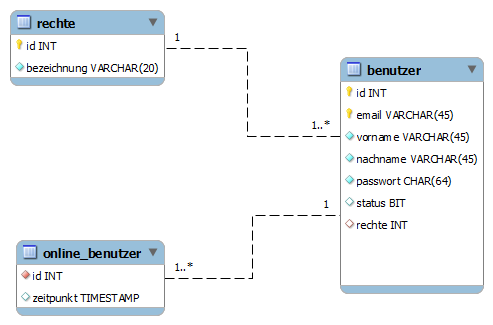
\includegraphics[scale = 0.6]{nutzerdatenbank} 
\caption [Entwurf Nutzerdatenbank]{Entwurf der Nutzerdatenbank}
\label{Nutzerdatenbank}
\end{figure} 

\newpage

\begin{itemize}
\item[1)] \textit{rechte:} 
In dieser Tabelle befinden sich sämtliche verfügbaren Rechte-Stufen, die sich aus einer eindeutigen ID und einer Bezeichnung in Textform zusammensetzen.

\item[2)] \textit{benutzer:} 
Alle registrierten Nutzer werden in dieser Tabelle gespeichert. Dabei besitzt jeder Nutzer eine eindeutige ID. Diese wird durch automatisches Inkrementieren von der Datenbank erzeugt. Mit der E-Mail-Adresse zusammen bilden beide den Primärschlüssel zur eindeutigen Identfikation eines Nutzers. Des Weiteren gehören zu einem Benutzereintrag noch ein Vor- und ein Nachname. Das vom Benutzer bei seiner Registrierung gewählte Passwort wird in gehashter Form als String gespeichert. Ein einzelnes Bit gibt zudem Auskunft darüber, ob der Nutzer bereits vom Vorstand aktiviert wurde und somit Zugang zu den Fahrzeugdaten erhalten hat. Das Feld "`rechte"\ ist Fremdschlüssel zur Tabelle "`rechte"\ und beinhaltet eine der dort befindlichen IDs.

\item[3)] \textit{online\_benutzer:} 
Diese Tabelle speichert Nutzer-IDs und Zeitstempel und gibt somit Auskunft über den Zeitpunkt der letzten Aktivität eines Nutzers.

\end{itemize}

\subsection{Fahrzeugdatenbank}

Die zweite Datenbank beinhaltet die aus dem Fahrzeug entnommen Daten und bildet gleichzeitig auch die Schnittstelle zur Webseite. Sie besteht aus fünf Tabellen, die jeweils sämtliche Informationen einer Kategorie in sich kapseln (s. Abb. \ref{Fahrzeugdatenbank}). Alle Tabellen besitzen über ihre Daten hinaus jeweils noch ein Feld, in dem sich ein Zeitstempel befindet und eines, das für Testzwecke Informationen speichern kann. Anhand des (im Fahrzeug erzeugten) Zeitstempels lassen sich die Datentupel der einzelnen Tabellen einander zuordnen. Im Folgenden werden die Informationen der einzelnen Tabellen erläutert:

\begin{figure}[h]
\centering
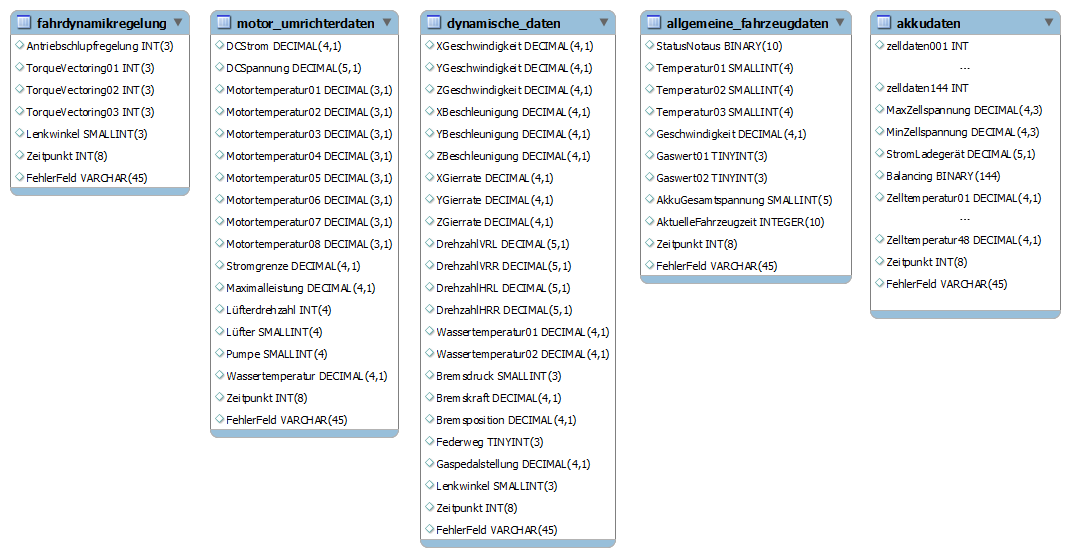
\includegraphics[scale = 0.43]{fahrzeugdatenbank} % Anm: neue Grafik!
\caption[Entwurf Fahrzeugdatenbank]{Entwurf der Fahrzeugdatenbank}
\label{Fahrzeugdatenbank}
\end{figure} 

\begin{itemize}

\item[1)] \textit{fahrdynamikregelung:} 
Diese Tabelle beinhaltet, wie der Name bereits verrät, alle Informationen bezüglich der Fahrdynamikregelung. Sie hält aktuelle Informationen über den Status der Antriebsschlupfregelung, dem Torque-Vectoring in x-, y- und z-Richtung sowie den Lenkwinkel.

\item[2)] \textit{motor\_umrichterdaten:}
Alle Daten, die den Motor und Umrichter betreffen, werden hier gespeichert. Informationen über den aktuell anliegenden Strom oder die aktuell anliegende Spannung sowie die Informationen aller acht Temperatursensoren des Motors lassen sich hier wiederfinden. Ebenso auch Informationen, die die Kühlung des Motors betreffen, wie Lüfterdrehzahlen, Pumpenleistung, Wassertemperatur und eingestellte Stromgrenzen.

\item[3)] \textit{dynamische\_daten:}
Alle Informationen, die die dynamischen Aspekte des Fahrzeugs betreffen, sind hier enthalten. Dies sind beispielsweise die Geschwindigkeiten, Be\-schleunigungen und Gierraten jeweils in x-, y- und z-Richtung, genau wie die Drehzahlen jedes einzelnen Rads. Desweiteren finden sich hier auch Informationen zu den Bremsen, wie Bremsdruck, -kraft und -position wieder. Auch der Lenkwinkel, der Federweg und die Gaspedalstellung ergänzen das Set der Daten.

\item[4)] \textit{allgemeine\_fahrzeugdaten:} 
Die wichtigsten und allgemeinsten Informationen des Fahrzeugs befinden sich in dieser Tabelle. Neben den wichtigen Informationen wie z.B. den Status der einzelnen Notaus-Schalter des Fahrzeuges, finden sich hier die Werte der drei wichtigsten Temperatursensoren, die aktuelle Fahrgeschwindigkeit, die Gaswerte der beiden Elektromotoren sowie die Gesamtspannung des Akkus und die aktuelle Fahrzeugzeit.

\item[5)] \textit{akkudaten:} Dies ist die letzte und zugleich auch die umfangreichste Tabelle. \\Hier befinden sich sämtliche Informationen über die im Fahrzeug verbauten Akkus. Neben globaleren Informationen wie die maximale und minimale Zellspannung und dem Strom bzw. der Spannung zum Ladegerät, finden sich die Zelldaten aller 144 Akkuzellen sowie die Temperaturen aller 48 Temperatursensoren wieder. Das Feld "`Balancing"\ gibt darüber hinaus Informationen darüber, ob für die einzelnen Zellen die Balancing-Option aktiviert oder deaktiviert ist.

\end{itemize}


\chapter{Testdrehbuch}

Im Folgenden wird der Ablauf der durchzuführenden Test geschildert. Dabei wird im ersten Teil darauf getestet, dass unter optimalen Umständen alle Funktionen korrekt ausgeführt werden. Im zweiten Teil wird anschließend das System auf dessen Robustheit geprüft, wobei auftretende Grenzfälle erkannt und korrekt behandelt werden sollen.


\section{Test auf Funktionalität}
\subsubsection*{
\hangindent+20pt \hangafter=1
I) In Matlab/Simulink werden Testwerte generiert, die innerhalb der vereinbarten Wertebereiche liegen \\}

\vspace*{3mm}

\textbf{1. /TM100/}
\hangindent+95pt \hangafter=1
\hspace*{5.5mm} 
Es wird geprüft, dass alle Daten korrekt gebündelt und an die Ethernet-Schnittstelle der MikroAutoBox II weitergeleitet werden. \\

\textbf{2. /TE120/TE300/}\\
\hangindent+95pt \hangafter=1
Am Embedded-PC wird der Empfang der Datenpakte überprüft.\\

\textbf{3. /TE100/}
\hangindent+95pt \hangafter=1
\hspace*{8mm} 
Bei einem Neustart durch Unterbrechung der Stromzufuhr des Embedded-PC soll dieser selbstständig die Verbindung zur MicroAutoBox II wiederaufbauen, sowie das GRPS/UMTS-Modul aktivieren und die Verbindung zum Webserver erneut etablieren.\\

\textbf{4. /TE200/}
\hangindent+95pt \hangafter=1
\hspace*{8mm} 
Die Signalqualität und Stabilität der GPRS/UMTS-Verbindung wird im Ruhezustand, bei Bewegung und bei großer Entfernung zum Sendemast bzw. bei schlechter Empfangsqualität überprüft.\\

\textbf{5. /TE300/}
\hangindent+95pt \hangafter=1
\hspace*{8mm}
Es wird zu TE200 auf dem virtuellen Server überprüft, ob die Testdaten vollständig und korrekt über eine GPRS/UMTS-Verbindung an ebendiesen übermittelt wurden. \\
 
\textbf{6. /TW200/}
\hangindent+95pt \hangafter=1
\hspace*{5.5mm} 
Nach mehr als 10 Stunden kontinuierlichen Datentransfers sollen die Fahrzeugdaten der letzten 10 Stunden in der Datenbank vorliegen. Den Ausgangspunkt für dieses Zeitintervall stellt den Zeitpunkt der Datenentnahme dar.\\
 
\textbf{7. /TW210/}
\hangindent+95pt \hangafter=1
\hspace*{5.5mm} 
Der korrekte Export der in der Datenbank enthaltenen Fahrzeugdaten als CSV-Datei wird auf dessen Fehlerfreiheit überprüft.\\

\textbf{8. /TW100/TW110/}\\
\hangindent+95pt \hangafter=1
Auf der Webseite wird die korrekte Visualisierung und Aufbereitung der Daten überprüft. Darin ist ebenfalls eine Überprüfung der fehlerfreien Darstellung auf den zuvor spezifizierten Browsern eingeschlossen. 

\newpage

\subsubsection*{
\hangindent+20pt \hangafter=1
II) Unabhängig davon können die Verwaltungsprozesse auf der Webseite überprüft werden:}

\vspace*{3mm}

\textbf{1. /TW440/}
\hangindent+95pt \hangafter=1
\hspace*{5.5mm}
Beim Aufrufen der Webseite wird der Nutzer zur Anmeldung \\ aufgefordert.\\

\textbf{2. /TW450/}
\hangindent+95pt \hangafter=1
\hspace*{5.5mm}
Bei einem nicht registrierten Nutzer schlägt der Anmeldeversuch fehl und eine Fehlermeldung wird ausgegeben (Nutzer nicht gefunden).\\

\textbf{3. /TW451/}
\hangindent+95pt \hangafter=1
\hspace*{5.5mm}
Ein registrierter Nutzer meldet sich mit E-Mail und Passwort an, ist aber noch nicht freigeschaltet (Status-Bit $==$ 0): Der Anmeldeversuch schlägt fehl und eine Fehlermeldung wird ausgegeben.(Nutzer noch nicht aktiviert)\\
 
\textbf{4. /TW452/}
\hangindent+95pt \hangafter=1
\hspace*{5.5mm}
Ein registrierten Nutzer meldet sich mit E-Mail und Passwort an.\\ (Status-Bit $==$ 1): der Vorgang verläuft ohne Fehler.\\
 
\textbf{5. /TW400/TW410/TW420/TW421/TW430/}\\
\hangindent+95pt \hangafter=1
Eine Registrierung mit E-Mail und Passwort (mind. 6 Zeichen) verläuft ohne Fehler. Der Nutzer wird daraufhin auf die Startseite weitergeleitet.\\

\textbf{6. /TW400/TW410/TW420/TW421/TW430/}\\
\hangindent+95pt \hangafter=1
Bei erfolgreichem Registrierungsversuch wird der Vorstand über das System per E-Mail  informiert und die Daten der Registrierung in die Nutzerdatenbank geschrieben. Das Status-Bit des Nutzers ist 0.\\

\textbf{7. /TW400/TW410/TW420/TW421/TW430/}\\
\hangindent+95pt \hangafter=1
Es wird darauf getestet, das beim Akzeptieren durch den Vorstand der Nutzer auch tatsächlich für die Anmeldung freigeschaltet wird. Das Status-Bit wird auf 1 gesetzt. Der Nutzer wird per E-Mail über dessen Freischaltung informiert. \\

\textbf{8. /TW400/TW410/TW420/TW421/TW430/}\\
\hangindent+95pt \hangafter=1
Es wird darauf getestet, dass beim Abweisen eines Registrierungsgesuches durch den Vorstand auch alle Daten des Registrierungsvorgangs aus der Nutzer-Datenbank gelöscht werden. \\

\textbf{9. /TW400/TW410/TW420/TW421/TW430/}\\
\hangindent+95pt \hangafter=1
Beim Zuweisen von Rechten an registrierte Nutzer werden diese Änderung korrekt in die Benutzerdatenbank übernommen.\\

\textbf{10. /TW460/}
\hangindent+95pt \hangafter=1
\hspace*{3.5mm}
Registrierte Nutzer, die mit Rechten ausgestattet wurden, können diese ohne Einschränkungen nutzen. \\

\newpage

\textbf{11. /TW421/}
\hangindent+95pt \hangafter=1
\hspace*{3.5mm}
Wird ein Nutzer durch den Vorstand gelöscht, so werden alle Daten zu diesem Nutzer aus der Nutzer-Datenbank gelöscht.\\

\textbf{12. /TW470/}
\hangindent+95pt \hangafter=1
\hspace*{2mm}
Wird die "`Passwort vergessen"\ - Funktion genutzt und eine E-Mail-Adresse eingegeben, die in der Benutzerdatenbank steht, dann wird eine E-Mail an die Adresse gesendet. Inhalt der E-Mail ist ein zufälliges Token, sowie ein Link zur Passwortänderung. \\

\textbf{13. /TW480/}
\hangindent+95pt \hangafter=1
\hspace*{2.5mm}
Es wird geprüft, ob der Link aus /TW470/ gültig ist und auf die Aktivierungsseite der Passwortwiederherstellung führt. \\

\textbf{14. /TW490/}
\hangindent+95pt \hangafter=1
\hspace*{2mm}
Wird auf der Aktivierungsseite der Passwortwiederherstellung die E-Mail-Adresse, das Token und das neue Passwort eingegeben, soll die Änderung korrekt in die Benutzerdatenbank übernommen werden.

\subsubsection*{
\hangindent+20pt \hangafter=1
III) Folgende Tests müssen auf dem virtuellen Server durchgeführt werden:}

\vspace*{3mm}

\textbf{1. /TS010/}
\hangindent+95pt \hangafter=1
\hspace*{6mm}
Die Dekodierung der vom Embedded-PC über eine GPRS/UMTS-Verbindung versendeten Datenpakete verläuft ohne Probleme. \\

\textbf{2. /TS020/}
\hangindent+95pt \hangafter=1
\hspace*{8mm}
Es wird anschließend getestet, ob die nunmehr dekodierten Datensätze anschließend korrekt aufbereitet werden (für die Durchführung der Aufbereitung s. 3.4.3). \\

\textbf{3. /TS030/}
\hangindent+95pt \hangafter=1
\hspace*{8mm}
Es wird darauf geprüft, dass bei längerer Laufzeit des Programms für die Paketverarbeitung der Speicherbedarf nicht unbegrenzt steigt.\\


\newpage


\section{Test auf Robustheit}
\subsubsection*{
\hangindent+20pt \hangafter=1
I) In Matlab/Simulink werden Testwerte generiert, die außerhalb der vereinbarten Wertebereiche liegen \\} 

\vspace*{3mm}

\textbf{1. /TR010/}
\hangindent+95pt \hangafter=1
\hspace*{8mm}
Das für die Plausibilitätsüberprüfung auf dem virtuellen Server zuständige Modul (s. 3.4.3) erkennt die Werte, welche außerhalb des Wertebereiches liegen und leitet diesbezüglich eine Warnmeldung an die Webseite weiter. \\

\textbf{2. /TR020/}
\hangindent+95pt \hangafter=1
\hspace*{5.5mm}
Auf der Webseite wird daraufhin die aufgetretene Überschreitung der Wertebereiche bei den jeweiligen Werten für den Nutzer kenntlich gemacht.



\subsubsection*{II) Tests auf der Webseite}

\vspace*{3mm}

\textbf{1. /TW400/TW410/TW420/TW421/TW430/}\\
\hangindent+95pt \hangafter=1
Eine Registrierung mit E-Mail und Passwort, welches weniger als 6 Zeichen aufweist, resultiert in einer Fehlermeldung.\\

\textbf{2. /TR030/}
\hangindent+95pt \hangafter=1
\hspace*{8mm}
Bei einer Anmeldung mit inkorrekter Email-Adresse und/oder falschem Passwort soll fehlschlagen und eine Fehlermeldung ausgegeben werden. \\

\textbf{3. /TR040/}
\hangindent+95pt \hangafter=1
\hspace*{6.5mm}
Meldet sich ein noch angemeldeter Nutzer erneut an, soll dies fehlschlagen und eine Statusmeldung über den aktuellen Zustand (angemeldet / nicht angemeldet) des Nutzers ausgegeben werden. \\

\textbf{4. /TR050/}
\hangindent+95pt \hangafter=1
\hspace*{5.5mm}
Falls dem Nutzer, nachdem er den "`Passwort vergessen"\ - Button ausgewählt hat, bei der Eingabe der E-Mail-Adresse zu Übersendung des Tokens und des Links zur Aktivierungsseite ein Fehler unterläuft, soll dies fehlschlagen und der Nutzer eine Statusmeldung darüber erhalten, dass seine eingegebene E-Mail-Adresse nicht im System existiert.  

\subsubsection*{
\hangindent+20pt \hangafter=1
III) Tests auf dem virtuellen Server:}

\textbf{1. /TS040/}
\hangindent+95pt \hangafter=1
\hspace*{6mm}
Wenn durch äußere Einflüsse das Programm zum Absturz gebracht wurde, soll sich dieses Neustarten lassen können.
%---------------------------  Glossar  -----------------------------%

\chapter*{Glossar}
\addcontentsline{toc}{chapter}{Glossar}

\textbf{Ajax}
\hangindent+75pt \hangafter=1
\hspace*{13.5mm}
Ajax ist ein Akronym für die Wortfolge "`Asynchronous JavaScript and XML". Es bezeichnet ein Konzept der asynchronen Datenübertragung zwischen einem Browser und dem Server.\\

\textbf{Apache-Server}
\hangindent+75pt \hangafter=1
\\
Apache (HTTP) Server bezeichnet eine modulare Webserversoftware.\\

\textbf{API}
\hangindent+75pt \hangafter=1
\hspace*{13.5mm}
Eine API (applictation programming interface) ist eine Programmierschnittstelle, die Funktionalitäten einer Software anderen Programmen zur Verfügung stellt.\\

\textbf{Architekturmuster} \\
\hangindent+75pt \hangafter=1 
Ein Architekturmuster ist eine aus Erfahrung entstandene und optimierte Schablone für häufig wiederkehrende Probleme, anhand derer man Software entwerfen kann.\\

\textbf{Balancing}
\hangindent+75pt \hangafter=1
\hspace*{3.5mm}
Der Begriff Balancer, zu deutsch (Zellen-Ladungszustands-) Ausgleicher oder Ausgleichsregler, bezeichnet ein elektrisches Gerät, das die gleichmäßige Ladung aller Zellen innerhalb eines Akkupacks gewährleistet.\\

\textbf{bidirektional}
\hangindent+75pt \hangafter=1 \\
Datenübertragung, die in beide Richtungen funktioniert. \\

\textbf{boolean}
\hangindent+75pt \hangafter=1 
\hspace*{7.5mm}
Ein Datentyp für die Darstellung der Werte "`wahr"\ und "`falsch".\\

\textbf{Browser}
\hangindent+75pt \hangafter=1
\hspace*{6.5mm}
Ein spezielles Computerprogramm, das für die Darstellung von Webseiten oder Daten verwendet wird.\\

\textbf{Busarray}
\hangindent+75pt \hangafter=1
\hspace*{5.5mm} 
Ein Busarray ist eine gebündelte und zusammengefasste Anzahl von Bussen.\\

\textbf{CAN-Bus}
\hangindent+75pt \hangafter=1
\hspace*{3mm} 
Der CAN-Bus (Controlled Area Network) ist ein asynchrones, serielles Bussystem und gehört zu der Klasse der Feldbusse.\\

\textbf{CSS}
\hangindent+75pt \hangafter=1
\hspace*{15mm}
Cascading Style Sheets sind eine deklarative Sprache für Stilvorlagen (engl. stylesheets) von strukturierten Dokumenten. Sie werden vor allem zusammen mit HTML eingesetzt.\\


\textbf{CSV}
\hangindent+75pt \hangafter=1
\hspace*{13.5mm}
Das Dateiformat CSV steht für den englischen Begriff Comma-separated values (gelegentlich auch Character-separated values) und beschreibt den Aufbau einer Textdatei zur Speicherung oder zum Austausch einfach strukturierter Daten.\\

\textbf{C++}
\hangindent+75pt \hangafter=1
\hspace*{13.5mm}
C++ ist eine objektorientierte Programmiersprache.\\

\textbf{Datenbank}
\hangindent+75pt \hangafter=1
\hspace*{1.25mm}
Eine Datenbank ermöglicht die permanente Speicherung von Daten. Die genaue Realisierung der Aufbewahrung wird von der Datenbank verwaltet, die Daten kann man mit speziellen Anfragen extrahieren.\\

\textbf{DC}
\hangindent+75pt \hangafter=1
\hspace*{16.5mm}
Die Abkürzung DC (direct current) steht für Gleichstrom.\\

\textbf{Dongle}
\hangindent+75pt \hangafter=1
\hspace*{8.75mm}
Ein Gerät (hier: USB-Stick), das an einen Computer o.ä. angeschlossen wird, um eine Verbindung zu kontrollieren. Dies dient zum Datenschutz und zur Kontrolle von gültigen Lizenzen.\\

\textbf{Embedded-PC} \\
\hangindent+75pt \hangafter=1 
Ein modular aufgebauter Industrierechner, dessen besonderer Fokus auf Kompaktheit liegt.\\

\textbf{Ethernet}
\hangindent+75pt \hangafter=1
\hspace*{5.5mm}
Übertragungstechnologie für Daten durch kabelgebundene Netze.\\

\textbf{Fremdschlüssel}
\hangindent+75pt \hangafter=1
\\
Eintrag in der Tabelle einer Datenbank dessen Inhalt nur Werte annehmen darf, die in einer definierten anderen Tabelle vorkommen.\\

\textbf{Gierrate}
\hangindent+75pt \hangafter=1
\hspace*{6.5mm}
Die Gierrate bezeichnet die Geschwindigkeit der Drehung eines Fahrzeugs um die Hochachse.\\

\textbf{GRPS}
\hangindent+75pt \hangafter=1
\hspace*{10.5mm}
Der General Packet Radio Service ist eine Übertragungstechnologie für die Mobilfunkübertragung von Daten (langsamer als UMTS).\\

\textbf{GPS}
\hangindent+75pt \hangafter=1
\hspace*{14mm}
Das Global Positiong System ist eine Technologie zur Positionsbestimmung und Zeitmessung.\\

\textbf{GUI}
\hangindent+75pt \hangafter=1
\hspace*{14.5mm}
Das Graphical User Interface (zu deutsch: Benutzeroberfläche) ist die grafische Schnittstelle zwischen Software und dem Benutzer.\\

\textbf{Hashing}
\hangindent+75pt \hangafter=1  
\hspace*{6.5mm}
Als Hashing bezeichnet man einen Vorgang, bei dem mittels einer Hashfunktion (auch Streufunktion) ein Eingabewert auf einen Ausgabewert abbildet. Man kann auf diese Weise sehr schnell an Daten kommen oder auch auf diese Weise Daten durch die Hashfunktion verschlüsselt speichern.\\

\textbf{HTML}
\hangindent+75pt \hangafter=1
\hspace*{9mm}
Die Hypertext Markup Language ist eine textbasierte Auszeichnungssprache zur Strukturierung von Inhalten wie Texten, Bildern und Hyperlinks in Dokumenten und im Internet.\\

\textbf{Interface}
\hangindent+75pt \hangafter=1
\hspace*{6mm}
Schnittstelle, über die Daten von verschiedenen Komponenten ausgetauscht werden können.\\

\textbf{IP}
\hangindent+75pt \hangafter=1
\hspace*{18.75mm}
Ein verbindungsloses Internetprotokoll, welches die Grundlage der Kommunikation im Internet darstellt.\\

\textbf{JavaScript}
\hangindent+75pt \hangafter=1
\hspace*{2.5mm}
JavaScript ist eine Skriptsprache, die hauptsächlich für dynamisches HTML in Webbrowsern eingesetzt wird. \\

\textbf{Latenz}
\hangindent+75pt \hangafter=1
\hspace*{10mm}
Laufzeit von Signalen, die sich aus der Differenz von dem Absenden und Ankommen von Daten ergibt.\\

\begin{spacing}{0.95} 

\textbf{Makro}
\hangindent+75pt \hangafter=1
\hspace*{9.75mm}
Ein Makro ist eine zusammengefasste Abfolge von Befehlen oder Deklarationen, die bei Aufruf sequentiell abgearbeitet werden.\\

\textbf{Matlab/Simulink} \\
\hangindent+75pt \hangafter=1 
Software, die hier verwendet wird, um die von der MicroAutoBox II bereitgestellten Daten zu verpacken und an den Embedded-PC weiterzuleiten.\\

\textbf{Matlab/Simulink-Block} \\
\hangindent+75pt \hangafter=1 
Mit der blockorientierten und graphischen Oberfläche von Simulink werden Gleichungen in Form von (Übertragungs-)Blöcken eingegeben und dargestellt.\\

\textbf{MicroAutoBox II} \\
\hangindent+75pt \hangafter=1 
Ein Echtzeitsystem, welches für schnelles Funktions-Prototyping in Fullpass- und Bypass-Szenarien geeignet ist.\\


\textbf{MySQL}
\hangindent+75pt \hangafter=1 
\hspace*{7.5mm}
MySQL ist eines der weltweit am weitesten verbreiteten relationalen Datenbankverwaltungssysteme. Es bildet die Grundlage für viele dynamische Webauftritte.\\

\textbf{MySQL Connector/C++}
\hangindent+75pt \hangafter=1
\\
Diese Software ermöglicht einen Zugriff auf eine MySQL-Datenbank. Dabei wird ein Programm in der Sprache C++ eingebunden.\\

\textbf{MySQL-Query}
\hangindent+75pt \hangafter=1 
\\
Eine für das MySQL-System geschriebene Anfrage in der Anfragesprache SQL zur Definition der gewünschten darzustellenden Datensätze.\\

\textbf{MySQL-Server}
\hangindent+75pt \hangafter=1
\\
Der MySQL-Server verwaltet die einzelnen Datenbanken und ermöglicht es, mehrere von diesen nebeneinander führen zu können. Es ist daher gleichzusetzen mit dem Begriff "`MySQL-Datenbankverwaltungssystem".\\

\textbf{Nutzersystem}
\hangindent+75pt \hangafter=1 \\
Verwaltung von Personen und deren Rechte im Rechtesystem.\\

%\textbf{Orgware}
%\hangindent+65pt \hangafter=1 
%\ \ Aus dem Englischen stammender Begriff, der die Rahmenbedingungen bei IT-Produkten und deren Projektabwicklung beschreibt.

\textbf{PHP}
\hangindent+75pt \hangafter=1
\hspace*{13.5mm}
PHP ist eine Skriptsprache, die hauptsächlich zur Erstellung dynamischer Webseiten oder Webanwendungen verwendet wird.\\

\textbf{PID-Regler}
\hangindent+75pt \hangafter=1 \\
Ein PID-Regler besteht aus 3 Teilen, einem P-Anteil, einem I-Anteil und einem D-Anteil. PI steht für proportional integral wirkend (wie beim PI-Regler) und D steht für differentiell wirkend.\\

\textbf{Port}
\hangindent+75pt \hangafter=1
\hspace*{14.2mm}
Der Port ist Bestandteil der Protokolle UDP und TCP.\\

\textbf{Primärschlüssel}
\hangindent+75pt \hangafter=1 \\
Primärschlüssel werden von Fremdschlüsseln referenziert. Dienen zur Eindeutigen Bestimmung von Tupeln in einer Tabelle.\\

\textbf{Recht}
\hangindent+75pt \hangafter=1 
\hspace*{11.5mm} Hier: Synonym für Erlaubnis.\\

\textbf{Rechtesystem}
\hangindent+75pt \hangafter=1 \\
Vergabe von Rechten für definierte Aktionen.\\

\textbf{Sampling}
\hangindent+75pt \hangafter=1 
\hspace*{4.5mm}
Sampling ist Englisch für "`Abtastung". Hierbei wird ein kontinuierliches Signal in festgelegten Zeitabständen abgetastet und der Wert bestimmt.\\

\textbf{Service-Interface} \\
\hangindent+75pt \hangafter=1 
Ein Service Interface ist eine Mensch-Fahrzeug-Schnittstelle, die es dem Menschen ermöglichen soll auf alle wichtigen Daten zuzugreifen.\\

\textbf{SFTP}
\hangindent+75pt \hangafter=1
\hspace*{11.25mm}
Das Secure File Transfer Protocol ist ein Protokoll, das es ermöglicht, über eine verschlüsselte Verbindung Daten zwischen zwei Geräten auszutauschen.\\

\textbf{Skript}
\hangindent+75pt \hangafter=1
\hspace*{10mm}
Ein Skript ist eine mit einer Skriptsprache wie PHP oder JavaScript geschriebene Datei, die von einem Programm ausgeführt werden kann.\\

\textbf{Smartphone}
\hangindent+75pt \hangafter=1 \\
Ein Smartphone (zu dt. intelligentes Telefon) beschreibt die aktuelle Gene\-ration von Mobilfunktelefonen, deren Eingabe auf einem berührungsempfindlichen Bildschirm erfolgt.\\

\end{spacing}

\textbf{Socket}
\hangindent+75pt \hangafter=1
\hspace*{10mm}
Ein Socket ist eine plattformunabhängige Schnittstelle, mit der man ein Netzwerkprotokoll implementieren kann. Dies ermöglicht es Rechnern, über Systemgrenzen hinweg miteinander zu kommunizieren.\\

\textbf{SSL/TLS}
\hangindent+75pt \hangafter=1
\hspace*{4.5mm}
Secure Sockets Layer/Transport Layer Security (zu Deutsch: Transportsicherheitsschicht) TLS ist die Weiterentwicklung von SSL, einem Protokoll zur verschlüsselten Datenübertragung im Internet.\\

\textbf{Tablet-PC}
\hangindent+75pt \hangafter=1 
\hspace*{3mm}
Ein tragbarer, flacher Computer in besonders leichter Ausführung mit einem Touchscreen-Display, wobei im Unterschied zu Notebooks auf eine physische Tastatur verzichtet wird.\\

\textbf{TCP/IP}
\hangindent+75pt \hangafter=1
\hspace*{6mm}
TCP/IP ist ein verbindungsorientiertes Kommunikationsprotokoll im Internet.\\

\textbf{Timeout}
\hangindent+75pt \hangafter=1
\hspace*{6mm}
Eine festgelegte Zeitgröße, die eine Aktion auslöst, wenn für einen mit dem Timeout festgelegten Zeitraum bestimmte Ereignisse ausgeblieben sind.\\

\textbf{Token}
\hangindent+75pt \hangafter=1 
\hspace*{12mm}
Ein Token dient als Sicherheitsmaßnahme zur zusätzlichen Authentifizierung einer Aktion im Internet (beispielsweise dem Setzen eines neuen Passworts) und besteht meist aus einer Aneinanderreihung von Buchstaben und Ziffern.\\

\textbf{Torque Vectoring}
\hangindent+75pt \hangafter=1 \\
Mit dem "`gezielt eingesetztem Drehmoment" (so die wörtliche Übersetzung von "`Torque Vectoring") lenkt das Fahrzeug noch spontaner und direkter in die Kurve ein, außerdem bleibt es deutlich länger spurstabil.\\

\textbf{Touchscreen} \\
\hangindent+75pt \hangafter=1 
{Ein Touchscreen (zu dt. berührungsempfindlcher Bildschirm) beschreibt einen Bildschirm, auf dem gleichzeitig Inhalte angezeigt werden können und Eingaben am Telefon durch Berührung erfolgen können.\\

\textbf{UDP}
\hangindent+75pt \hangafter=1
\hspace*{13mm}
UDP ist ein verbindungsloses Protokoll für Datenübertragungen zwischen zwei Anwendungen durch ein Netzwerk hindurch.\\

\textbf{UDP-Paket}
\hangindent+75pt \hangafter=1
\hspace*{0mm}
UDP zerlegt die zu verschickenden Daten in einzelne Datenpakete, die dann mit Zusatzinformationen versehen verschickt werden.\\

\textbf{UML}
\hangindent+75pt \hangafter=1
\hspace*{13mm}
Unified Modeling Language (dt. Vereinheitlichte Modellierungssprache)  ist eine standardisierte, graphische Modellierungssprache, die zur Spezifikation, Aufbau und Konstruktion von Software genutzt wird. In ihr enthalten sind aufgrund der Vielfältigkeit von Softwareproblemen viele verschiedene Diagrammtypen, die sich zur Problembeschreibung beziehungsweise deren Lösung unterschiedlich gut eignen.\\

\textbf{Umrichter}
\hangindent+75pt \hangafter=1
\hspace*{2.5mm}
Hierbei handelt es sich um einen Stromrichter, der aus einer Wechselspannung eine in der Frequenz und Amplitude unterschiedliche Wechselspannung generiert.\\

\textbf{UMTS}
\hangindent+75pt \hangafter=1
\hspace*{10.5mm}
Universal Mobile Telecommunications System ist eine Übertragungstechnologie für die Mobilfunkübertragung von Daten (schneller als GPRS).\\

\textbf{virtueller Server}
\hangindent+75pt \hangafter=1
\\
Eine Servervirtualisierung ist eine Softwarelösung, um mehrere virtuelle Server (auch vServer) auf einer Servermaschine laufen zu lassen. Dabei wird nur vorgegeben, dass der virtuelle Server ein richtiger Server ist, der getrennt von den anderen Instanzen läuft. Man kann den virtuellen Server allerdings wie einen normalen behandeln. Bei dem unserem Team vorliegenden vServer wird vom Provider 1\&1 das Betriebssystem Cent OS 6 emuliert.\\

\textbf{Voyage Linux}
\hangindent+75pt \hangafter=1
\\
Voyage Linux ist ein Debian-basiertes Linux-Betriebssystem für einen Embedded-PC.\\


%\textbf{Webspace}
%\hangindent+65pt \hangafter=1
%Als Webspace wird der bei einem Anbieter gemietete, aus dem Internet zugängliche Speicher bezeichnet, der für die Aufbewahrung von Daten und Webseiten verwendet wird.\\

\textbf{Webseite}
\hangindent+75pt \hangafter=1
\hspace*{6mm}
Eine Webseite ist ein meist interaktives Dokument, das auf einem Webserver liegt und aus dem Internet erreichbar ist.\\

\textbf{Webserver}
\hangindent+75pt \hangafter=1
\hspace*{2mm}
Ein Webserver ist ein Computer mit einer Serversoftware, der Dokumente beispielsweise an Webbrowser übermittelt.\\

\textbf{weiche Echtzeit}
\hangindent+75pt \hangafter=1 \\
Das System soll Daten in einem festgelegten Zeitrahmen zur Verfügung stellen, es muss aber nicht gewährleistet werden, dass es das immer tut.\\

%----------------------  Abbildungsverzeichnis  --------------------%

\listoffigures

\addcontentsline{toc}{chapter}{Abbildungsverzeichnis}
%
%---------------------------  Anhang  ------------------------------%

%\addcontentsline{toc}{chapter}{Anhang}

\appendix
\addchap{Anhang} 
\refstepcounter{chapter}

\section{Datentypen in Simulink}

Simulink unterstützt die folgenden von Matlab unterstützen Datentypen:

\begin{itemize}

\item \textit{double} (double-precision floating point nach IEEE Standard 754 mit 64 bit Speicherbedarf pro Zahl)

\item \textit{single} (single-precision floating point nach IEEE Standard 754 mit 32 bit Speicherbedarf pro Zahl)

\item \textit{int8, uint8, int16, uint16, int32, uint32} (signed/unsigned 8-, 16- bzw. 32-bit integer)

\end{itemize}

Darüber hinaus kennt Simulink noch den Datentyp

\begin{itemize}

\item \textit{boolean} (0 oder 1, wird intern als \textit{uint8} behandelt)

\end{itemize} 
\hangindent+40pt \hangafter=1
\textit{Quelle:} Angermann | Beuschel | Rau | Wohlfahrt: \\         "` MATLAB - Simulink - Stateflow: Grundlagen, Toolboxen, Beispiele"\ \\
Oldenbourg Verlag München


\section{Datentypen (Titel überarbeiten)}

Folgende Datentypen kommen in C++ oder MySQL-Datenbanken zu den bereits oben genannten Typen hinzu:

\begin{itemize}

\item Ganzzahldatentypen: \textit{decimal, smallint, tinyint} (nach Genauigkeit absteigend sortiert)

\item zeichenbasierte Datentypen: \textit{char} (Abspeicherung eines Zeichens), \textit{String} (Abspeicherung einer Zeichenfolge), \textit{varchar} (Datenbankenäquivalent zu \textit{String}), \textit{binary} (Abspeicherung einer Kette von Binärwerten)

\end{itemize}

Weiterhin kann eine MySQL-Datenbank noch folgenden Datentyp behandeln:

\begin{itemize}

\item \textit{bit} (Speicherung einer Binärzahl)

\end{itemize}


\section{UML-Diagramme}

\begin{sidewaysfigure}[t]
\centering
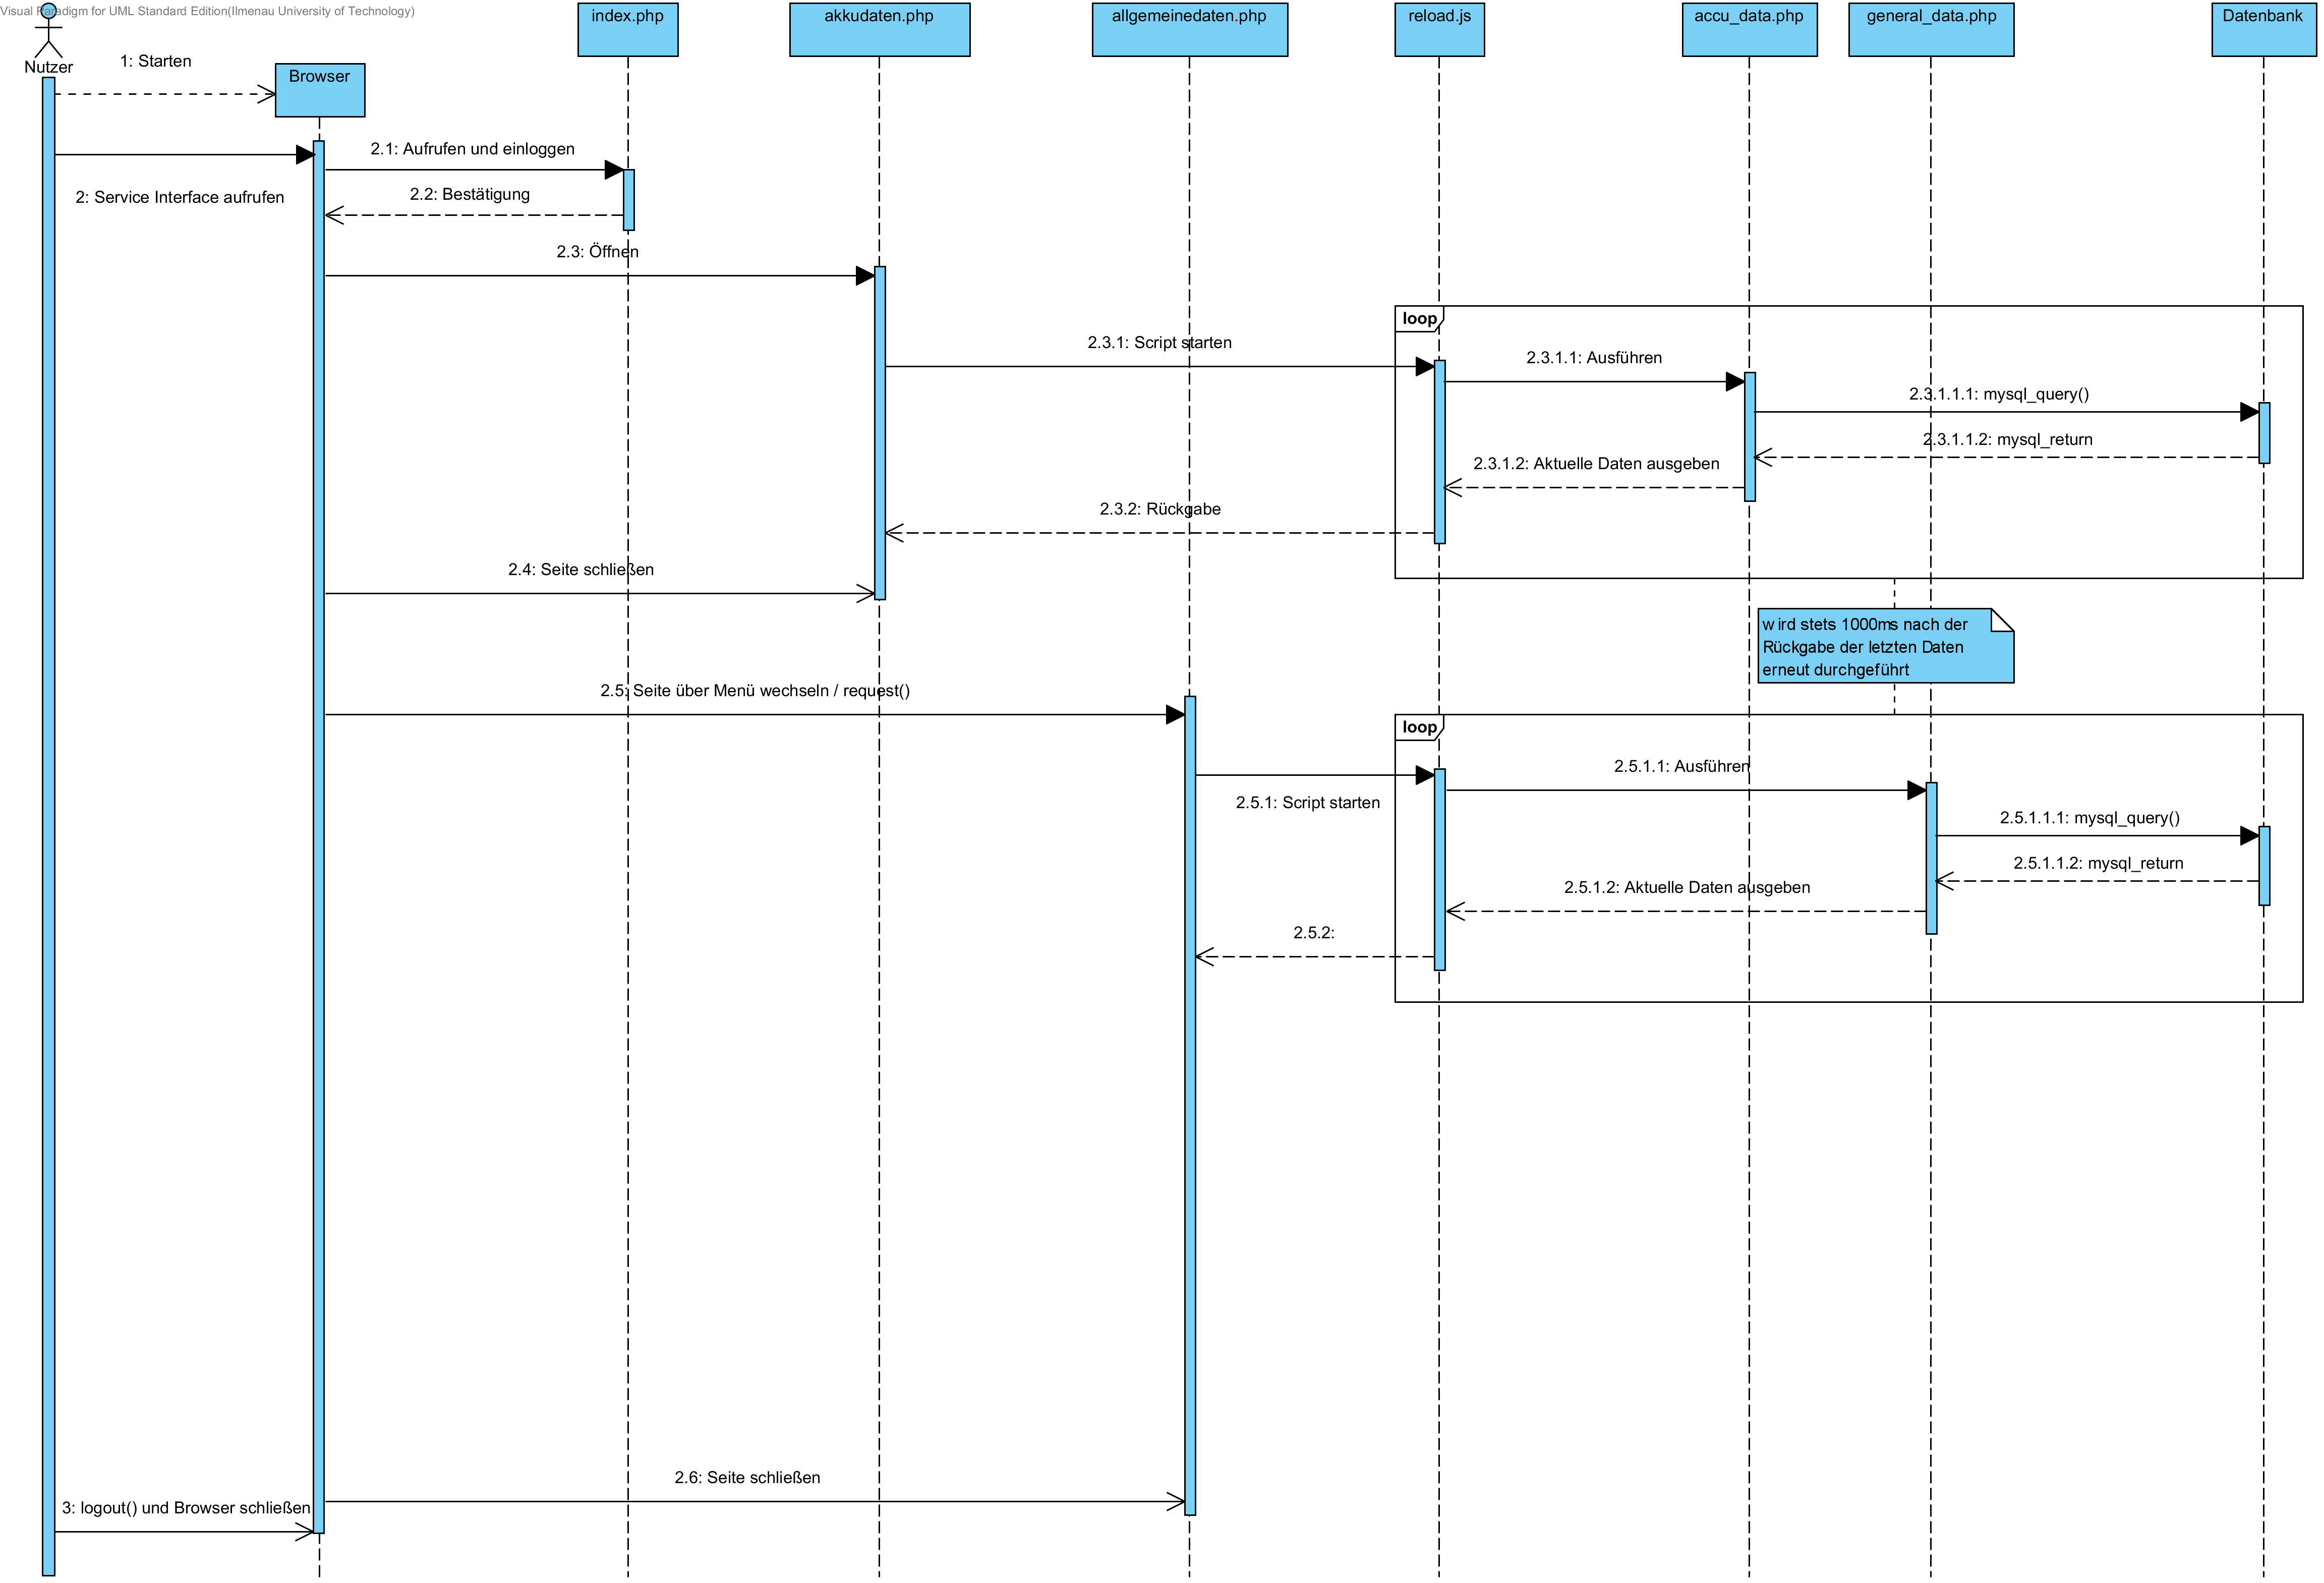
\includegraphics[scale = 0.55]{webseite}
\caption[Sequenzdiagramm Webseite]{Sequenzdiagramm der Webseite}
\end{sidewaysfigure} 

\newpage

\begin{sidewaysfigure}[t]
\centering
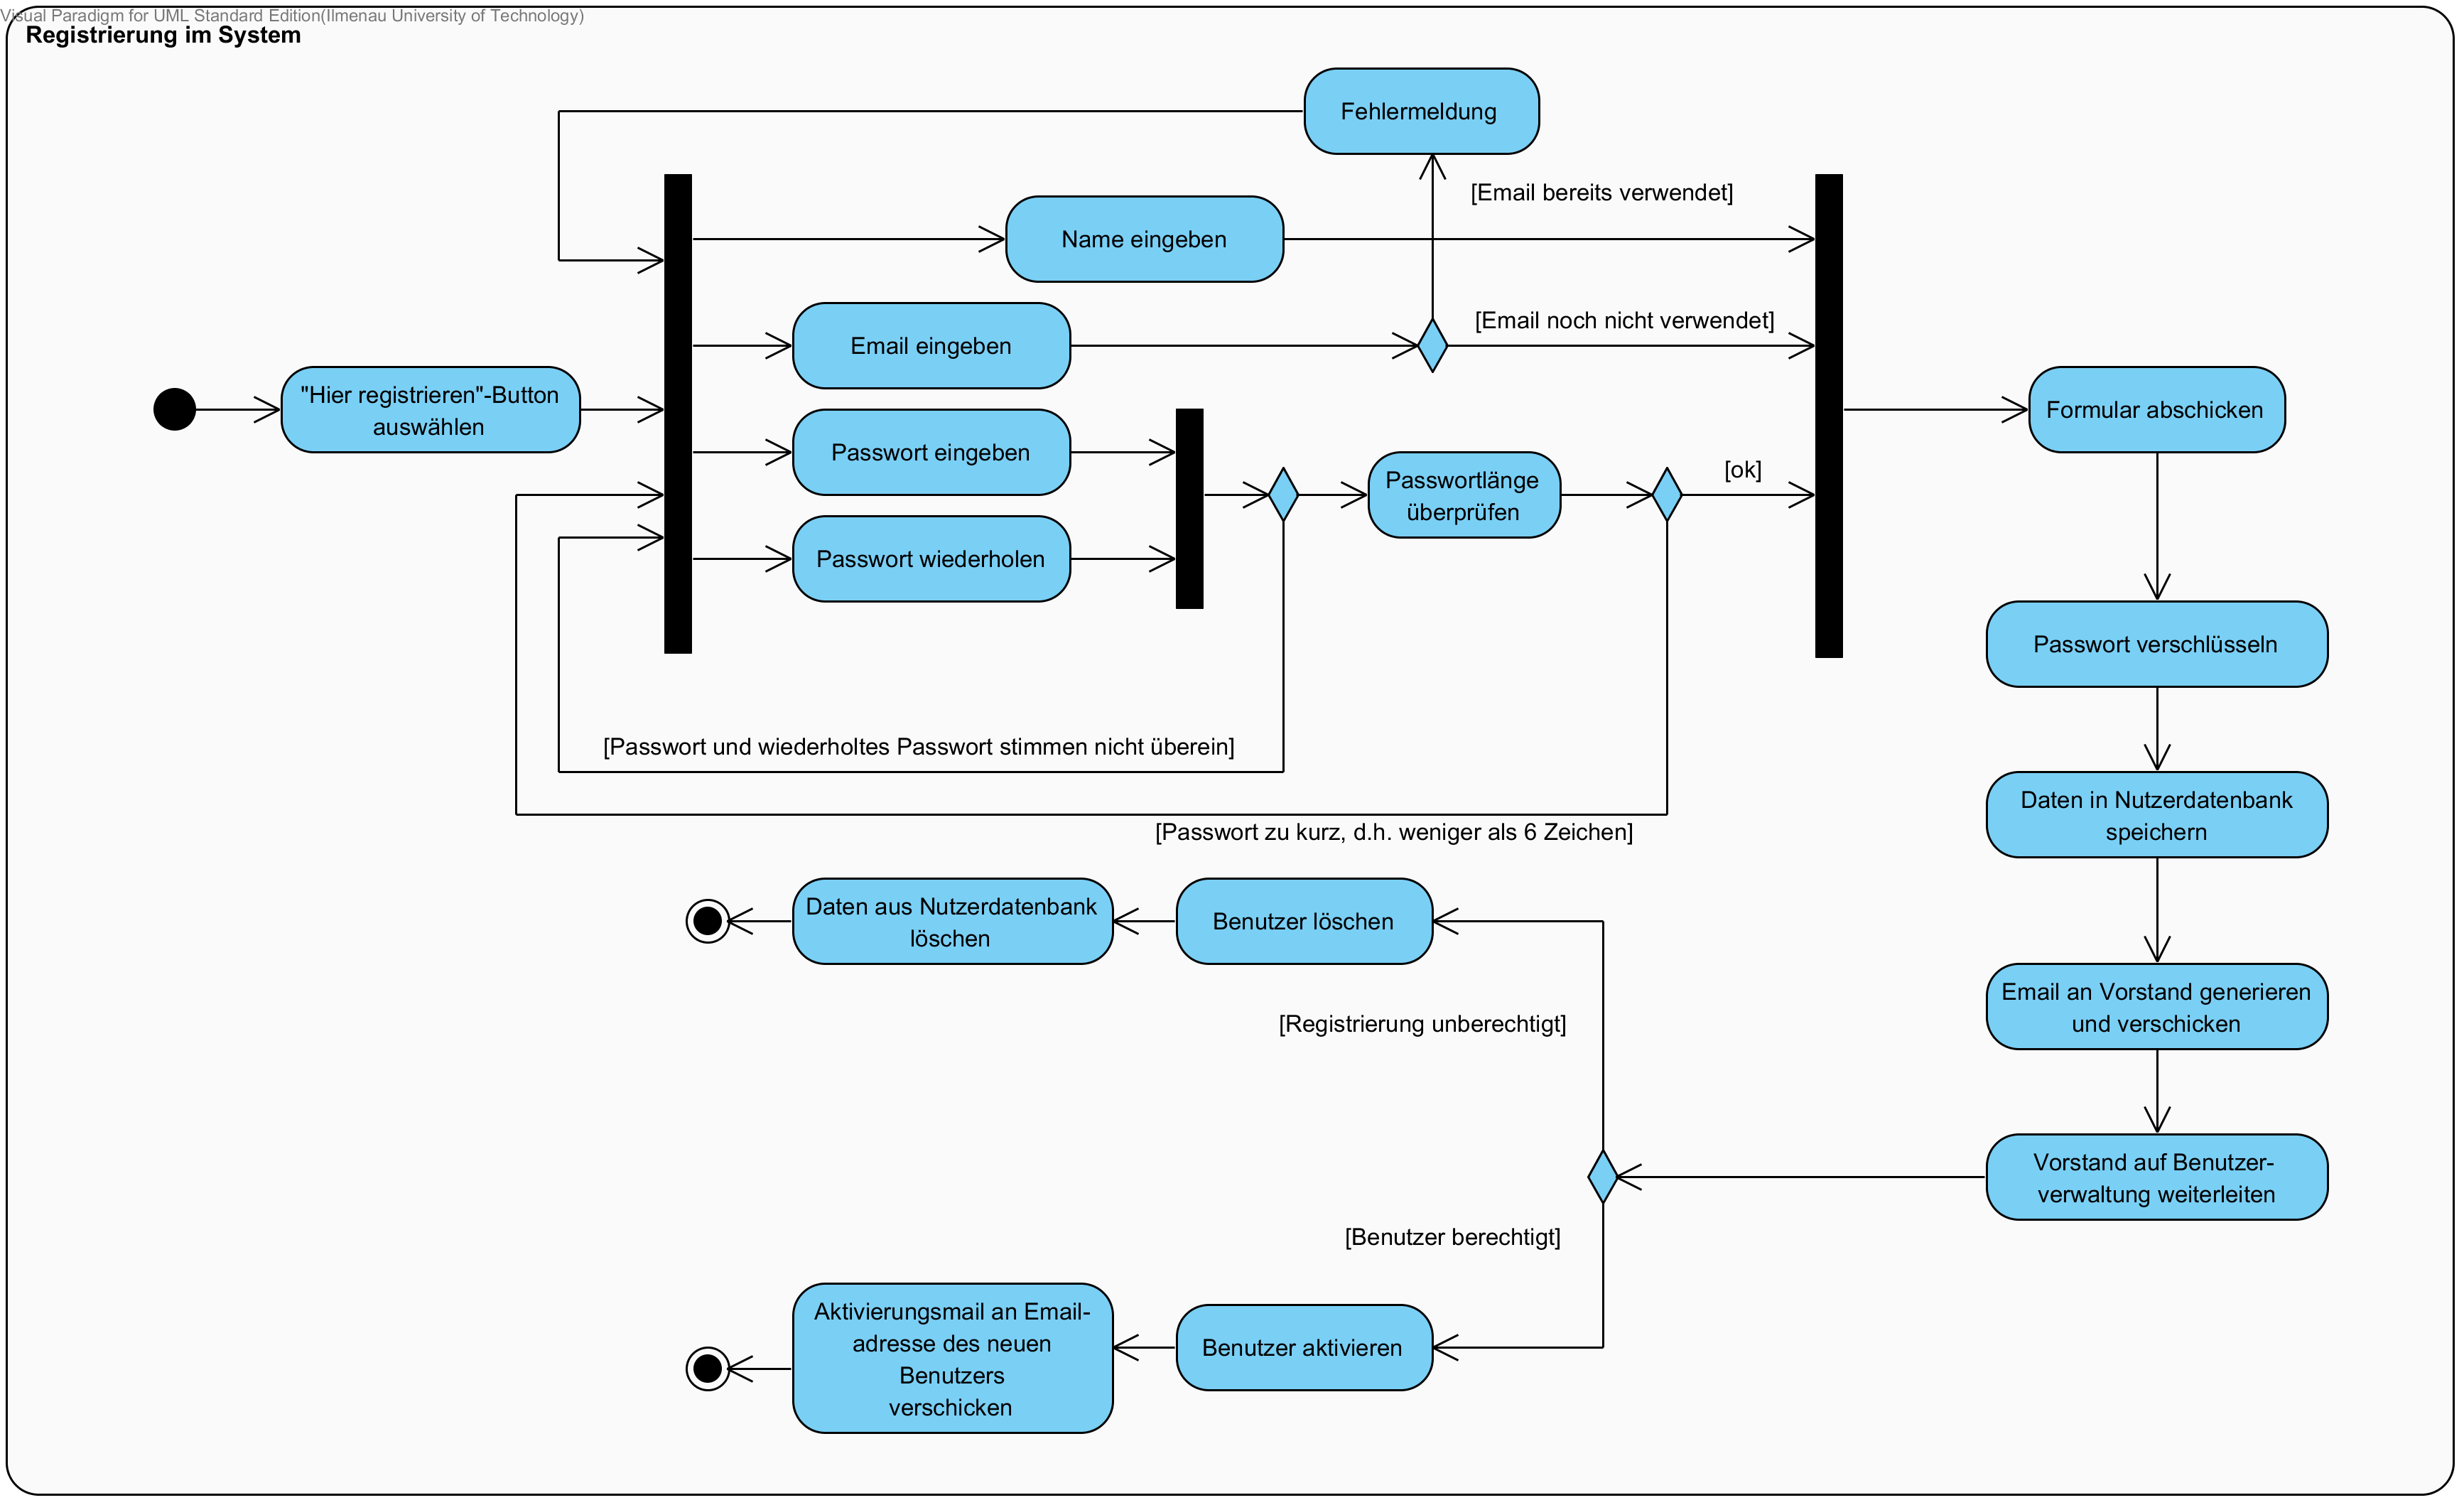
\includegraphics[scale = 0.75]{registrierungsvorgang}
\caption[Aktivitätsdiagramm Registrierungsvorgang]{Aktivitätsdiagramm des Registrierungsvorgangs}
\end{sidewaysfigure} 

\newpage

\end{document}